%%%%%%%%%%%%%%%%%%%%%%%%%%%%%%%%%%%%%%%%%%  不使用 authblk 包制作标题  %%%%%%%%%%%%%%%%%%%%%%%%%%%%%%%%%%%%%%%%%%%%%%
%-------------------------------PPT Title-------------------------------------
\title{计算材料团队工作简介}
%-----------------------------------------------------------------------------

%----------------------------Author & Date------------------------------------
%\author[\textrm{Jun\_Jiang}]{姜\;\;骏\inst{}} %[]{} (optional, use only with lots of authors)
%% - Give the names in the same order as the appear in the paper.
%% - Use the \inst{?} command only if the authors have different
%%   affiliation.
\institute[BCC]{\inst{}%
%\institute[Gain~Strong]{\inst{}%
\vskip 2pt 北京市计算中心~云平台事业部~材料计算团队}
%\vskip -20pt {\large 格致斯创~科技}}
\date[\today] % (optional, should be abbreviation of conference name)
{	%{\fontsize{6.2pt}{4.2pt}\selectfont{\textcolor{blue}{E-mail:~}\url{jiangjun@bcc.ac.cn}}}
\vskip 20 pt {\fontsize{8.2pt}{6.2pt}\selectfont{%清华大学\;\;物理系% 报告地点
	\vskip 5 pt \textrm{2025.03.20}}}
}

%% - Either use conference name or its abbreviation
%% - Not really information to the audience, more for people (including
%%   yourself) who are reading the slides onlin%%   yourself) who are reading the slides onlin%%   yourself) who are reading the slides onlineee
%%%%%%%%%%%%%%%%%%%%%%%%%%%%%%%%%%%%%%%%%%%%%%%%%%%%%%%%%%%%%%%%%%%%%%%%%%%%%%%%%%%%%%%%%%%%%%%%%%%%%%%%%%%%%%%%%%%%%

\subject{}
% This is only inserted into the PDF information catalog. Can be left
% out.
%\maketitle
\frame
{
%	\frametitle{\fontsize{9.5pt}{5.2pt}\selectfont{\textcolor{orange}{“大数据中心调研座谈会”}}}
\titlepage
}
%-----------------------------------------------------------------------------

%------------------------------------------------------------------------------列出全文 outline ---------------------------------------------------------------------------------
\section*{}
\frame[allowframebreaks]
{
  \frametitle{Outline}
%  \frametitle{\textcolor{mycolor}{\secname}}
  \tableofcontents%[current,currentsection,currentsubsection]
}
%%在每个section之前列出全部Outline
%%类似的在每个subsection之前列出全部Outline是\AtBeginSubsection[]
%\AtBeginSection[]
%{
%  \frame<handout:0>%[allowframebreaks]
%  {
%    \frametitle{Outline}
%%全部Outline中,本部分加亮
%    \tableofcontents[current,currentsection]
%  }
%}

%-----------------------------------------------PPT main Body------------------------------------------------------------------------------------
\small
\section{团队简介}
\frame
{
	\frametitle{团队概况}
	计算材料团队成立于\textrm{2016}年
	\vskip 2pt 
	自\textrm{2017}年起,团队承担国家重点研发计划\textcolor{magenta}{``材料基因工程关键技术与支撑平台''}项目相关研究任务,包括
\begin{itemize}
		\item \textcolor{blue}{高通量并发式材料计算算法和软件}
		\item \textcolor{blue}{高通量材料计算的工作流设计与交互图形化}
		\item \textcolor{blue}{材料基因工程数据汇交与管理服务技术平台}
	\end{itemize}
%	\frametitle{近期研究任务}
	\vskip 2pt
	自\textrm{2024}年起,团队与北京航空航天大学、北京科技大学、中科院宁波材料所等科研单位合作,联合承担的在研项目包括
\begin{itemize}
	\item \textcolor{blue}{国家自然基金面上项目}:\\
低维材料等离和激子极化激元的第一性原理研究%(项目编号: 12474217)}
	\item \textcolor{blue}{科技部重大专项}:\\
			基于人工智能技术的高性能多尺度分子动力学模拟平台%(项目编号: 2024ZD0606900)
	\end{itemize}
}
	
\frame
{
\frametitle{科研定位}
	经过数年探索,团队确立了\textcolor{purple}{以人工智能和数据为主要驱动力,面向基础科学中的应用研究问题}的指导思想,主要围绕
	\begin{itemize}
	 \setlength{\itemsep}{3pt}
		\item 微观尺度计算材料平台建设、第一原理计算方法与算法研究
		\item 结合机器学习方法和人工智能,对金属氧化物、半导体和合金材料的电子结构和热力学性质进行理论计算,形成材料数据库
		\item \textrm{AI for Scienece}:~化学-化工知识图谱与垂直领域模型的构建
		\item 应用型材料基础科学研究\\
	{\fontsize{7.2pt}{6.2pt}\selectfont{
		金属慢化反应堆中氢化锆的分子动力学模拟(\textcolor{blue}{新近开展})\\
		金属催化\textrm{\ch{CO2}}还原的机理研究(\textcolor{blue}{新近开展})}}
	\end{itemize}
	等方向展开研究,取得了一些研究成果
}

\frame
{
	\frametitle{团队成员}
\begin{figure}[h!]
\vspace*{-0.10in}
\centering
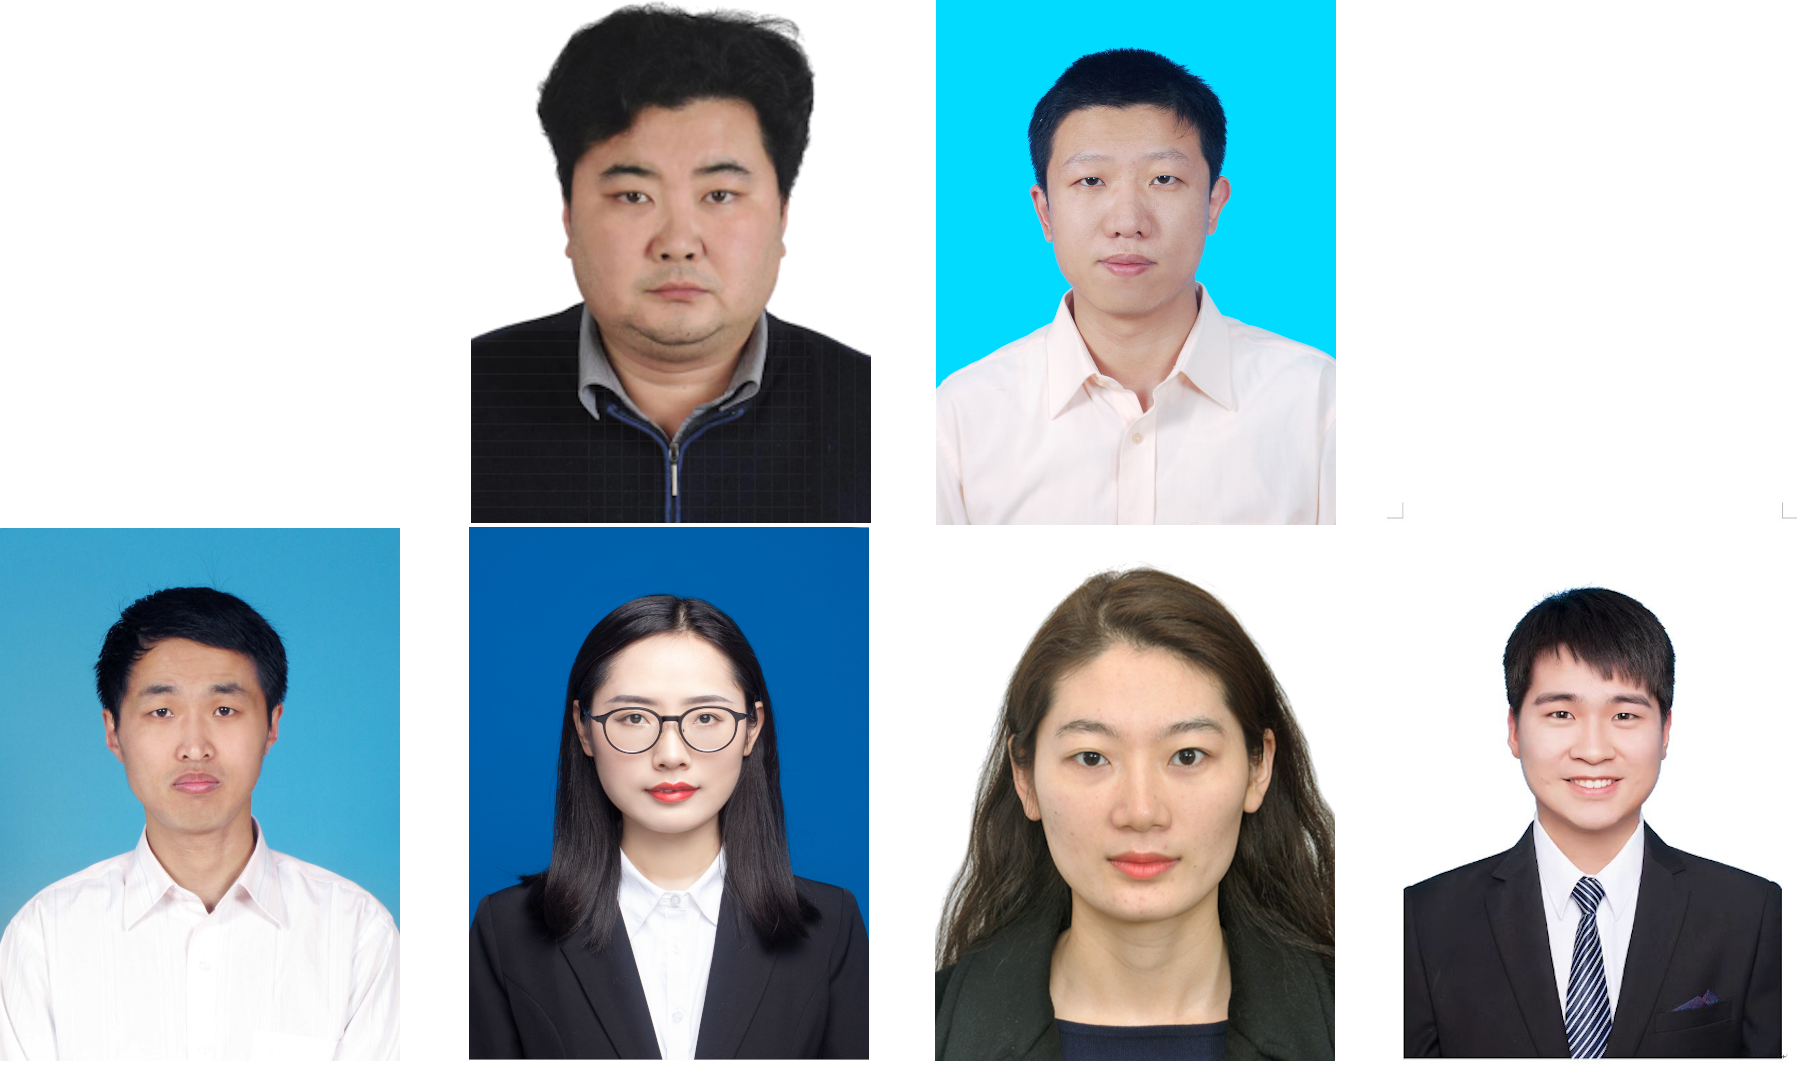
\includegraphics[height=2.40in,width=4.00in,viewport=0 0 430 270,clip]{Figures/Team_Member.png}
%\caption{\tiny \textrm{Pseudopotential for metallic sodium, based on the empty core model and screened by the Thomas-Fermi dielectric function.}}%(与文献\cite{EPJB33-47_2003}图1对比)
\label{Team_Membwe}
\end{figure}
}

\section{研究背景}
\frame
{
	\frametitle{科学研究的范式变更}
\begin{figure}[h!]
\vspace*{-0.28in}
\centering
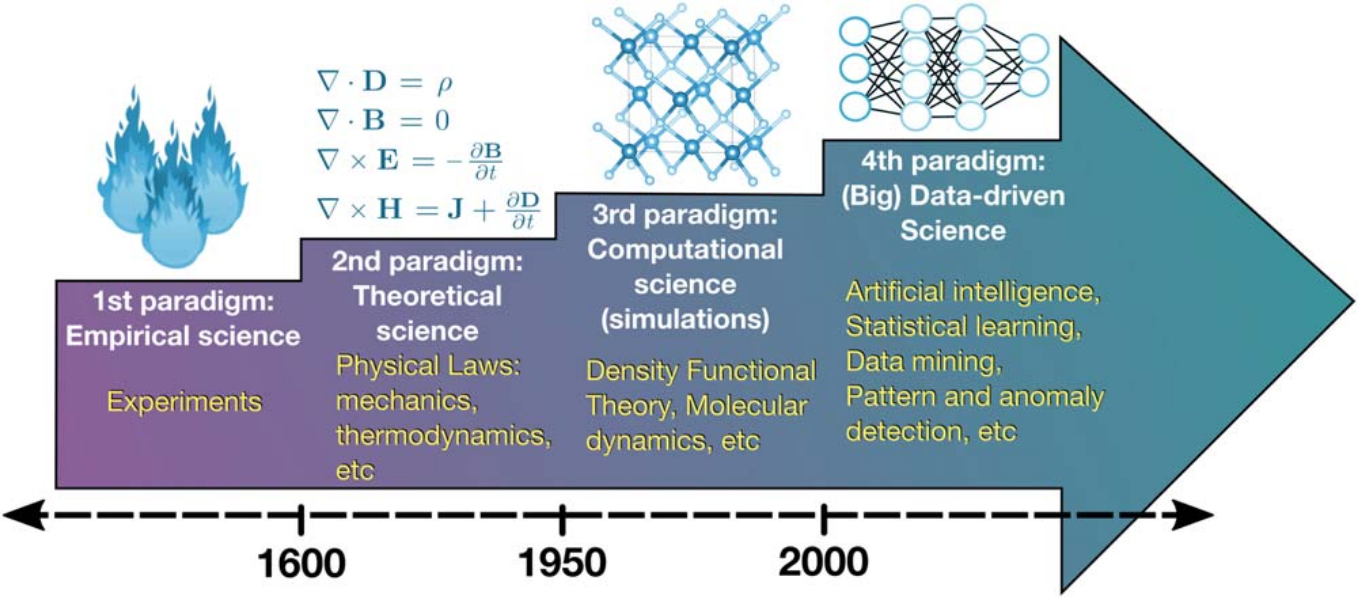
\includegraphics[height=2.00in,width=4.15in]{Figures/Four_Model_3.png}
%\caption{\tiny \textrm{Pseudopotential for metallic sodium, based on the empty core model and screened by the Thomas-Fermi dielectric function.}}%(与文献\cite{EPJB33-47_2003}图1对比)
\label{Four_Model}
\end{figure}
\begin{minipage}[b]{0.48\textwidth}
 {\fontsize{7.5pt}{6.0pt}\selectfont\begin{itemize}%[+-| alert@+>]
	 \setlength{\itemsep}{10pt}
 \item 逐步趋于理性
 \item 逐步趋于复杂
 \end{itemize}}
\end{minipage}
\hfill
\begin{minipage}[b]{0.48\textwidth}
 {\fontsize{7.5pt}{6.0pt}\selectfont\begin{itemize}%[+-| alert@+>]
	 \setlength{\itemsep}{10pt}
 \item 逐步趋于抽象
 \item 逐步趋于深刻
 \end{itemize}}
\end{minipage}
}

\begin{frame}{科学研究的重要助手:~计算模拟}
\begin{figure}[h!]
\vspace*{-0.18in}
\centering
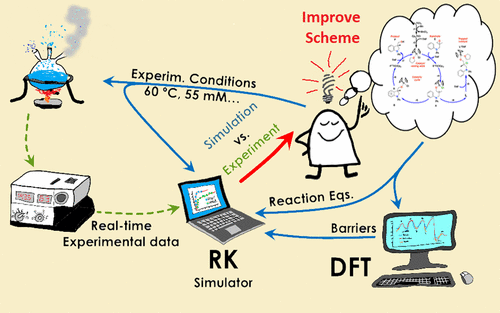
\includegraphics[height=2.55in,width=4.05in]{Figures/Schematic_Material-Design.png}
%\caption{\tiny \textrm{Pseudopotential for metallic sodium, based on the empty core model and screened by the Thomas-Fermi dielectric function.}}%(与文献\cite{EPJB33-47_2003}图1对比)
%\caption{\tiny \textrm{Pseudopotential for metallic sodium, based on the empty core model and screened by the Thomas-Fermi dielectric function.}}%(与文献\cite{EPJB33-47_2003}图1对比)
\label{Schematic_Material-Design}
\end{figure}
\end{frame}

\frame
{
	\frametitle{材料模拟的基本思想和方法}
\begin{figure}[h!]
\vspace*{-0.25in}
\centering
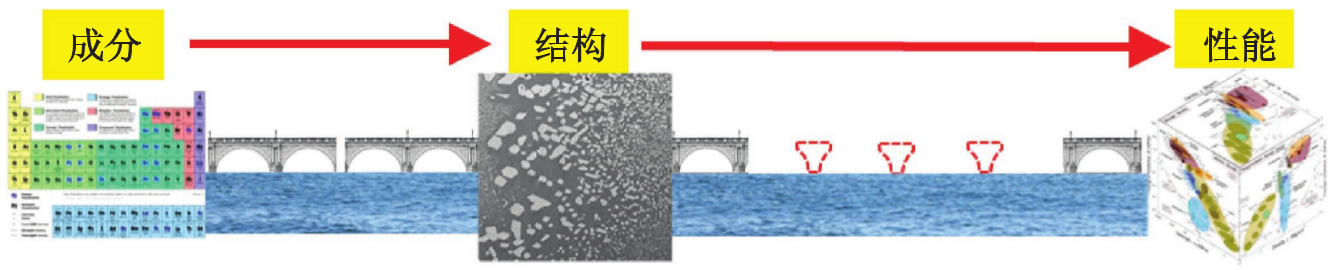
\includegraphics[height=0.80in,width=4.05in]{Figures/MGE-2.png}
%\caption{\tiny \textrm{Pseudopotential for metallic sodium, based on the empty core model and screened by the Thomas-Fermi dielectric function.}}%(与文献\cite{EPJB33-47_2003}图1对比)
\label{MGE}
\end{figure}
\begin{minipage}[c]{0.30\textwidth}
\begin{itemize}%[+-| alert@+>]
\vspace*{-2.25in}
 {\fontsize{7.5pt}{6.0pt}\selectfont
	 \setlength{\itemsep}{10pt}
 \item 变革研发模式,计算-实验-理论-数据科学相融合: 高效、低耗按需设计
 \item 数据驱动的材料创新平台主要面向复杂材料的模拟}
 \end{itemize}
\end{minipage}
\hfill
\begin{minipage}[b]{0.68\textwidth}
\begin{figure}[h!]
%\vspace*{-0.25in}
\centering
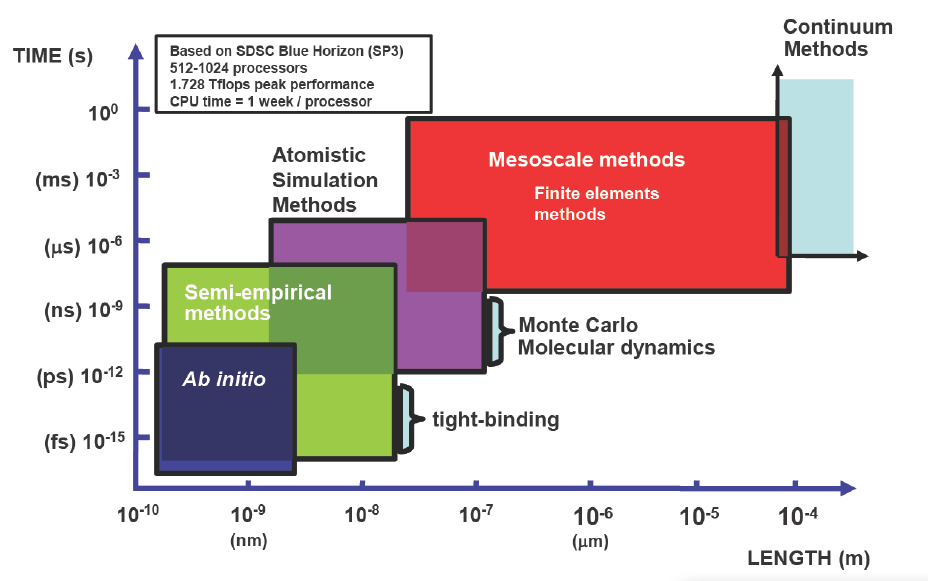
\includegraphics[height=1.80in,width=2.75in]{Figures/Multi-Scale-6.png}
%\caption{\tiny \textrm{Pseudopotential for metallic sodium, based on the empty core model and screened by the Thomas-Fermi dielectric function.}}%(与文献\cite{EPJB33-47_2003}图1对比)
\label{Multi-Scale}
\end{figure}
\end{minipage}
}

\frame
{
	\frametitle{数据驱动的科学研究}
前所未有的计算能力和大规模的数据收集能力%,现代科学正在进入“第四范式”:
\begin{figure}[h!]
%\vspace*{-0.05in}
\centering
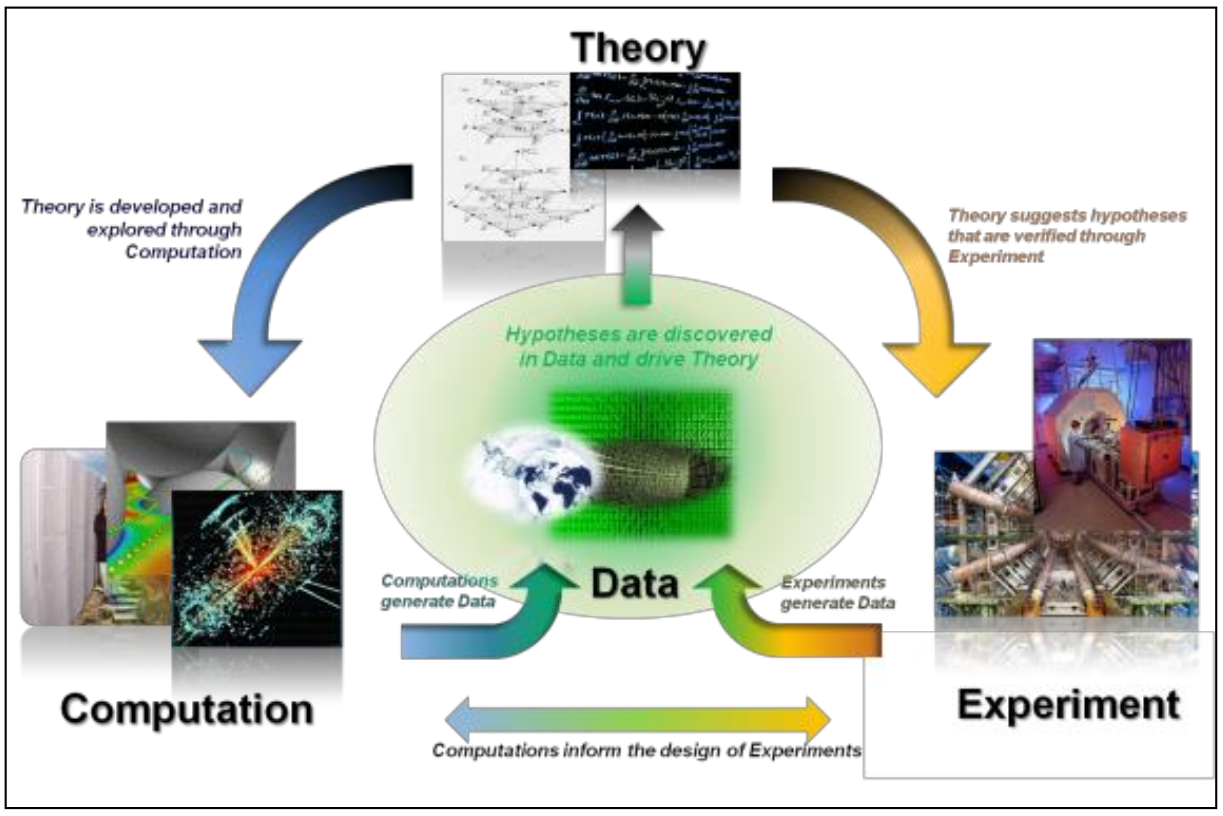
\includegraphics[height=2.30in,width=3.70in]{Figures/Four_Model_1.png}
%\caption{\tiny \textrm{Pseudopotential for metallic sodium, based on the empty core model and screened by the Thomas-Fermi dielectric function.}}%(与文献\cite{EPJB33-47_2003}图1对比)
\label{Four_Model_1}
\end{figure}
科学的新驱动力:~\textcolor{red}{密集数据}+\textcolor{red}{人工智能}\\
}

\frame
{
	\frametitle{材料基因工程}
\begin{figure}[h!]
\vspace*{-0.18in}
\centering
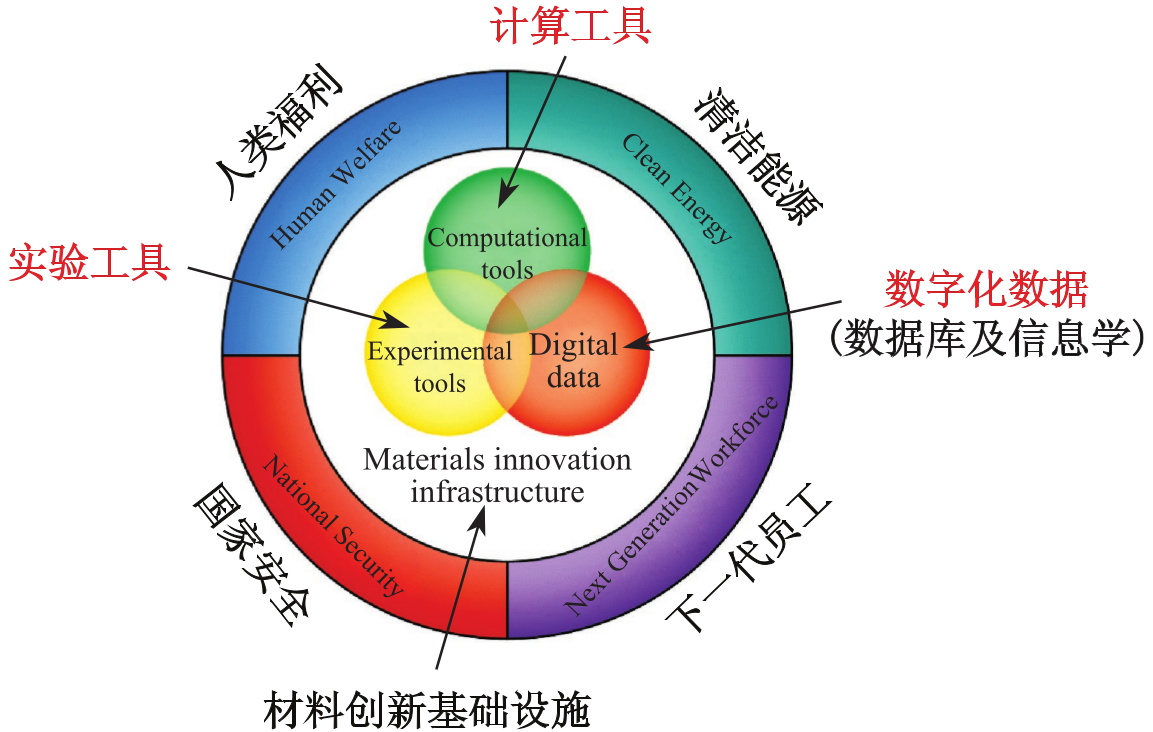
\includegraphics[height=2.55in,width=4.05in]{Figures/MGE.png}
%\caption{\tiny \textrm{Pseudopotential for metallic sodium, based on the empty core model and screened by the Thomas-Fermi dielectric function.}}%(与文献\cite{EPJB33-47_2003}图1对比)
%\caption{\tiny \textrm{Pseudopotential for metallic sodium, based on the empty core model and screened by the Thomas-Fermi dielectric function.}}%(与文献\cite{EPJB33-47_2003}图1对比)
\label{MGE}
\end{figure}
}

\begin{frame}
	\frametitle{材料基因工程推动新材料发展}
\begin{figure}[h!]
\vspace*{-0.25in}
\centering
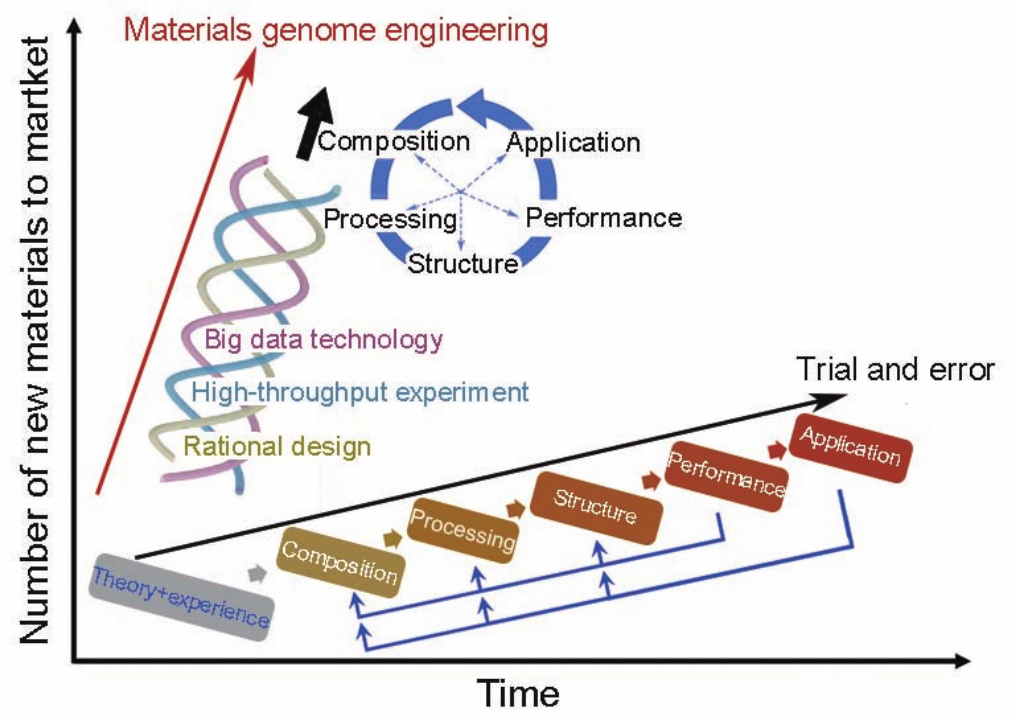
\includegraphics[height=2.90in,width=4.80in,viewport=0 0 1250 710,clip]{Figures/MGE_idea.png}
%\caption{\tiny \textrm{Pseudopotential for metallic sodium, based on the empty core model and screened by the Thomas-Fermi dielectric function.}}%(与文献\cite{EPJB33-47_2003}图1对比)
\label{MGE_idea}
\end{figure}
\end{frame}

%\begin{frame}
%	\frametitle{理论、方法与软件}
%\begin{figure}[h!]
%\vspace*{-0.25in}
%\centering
%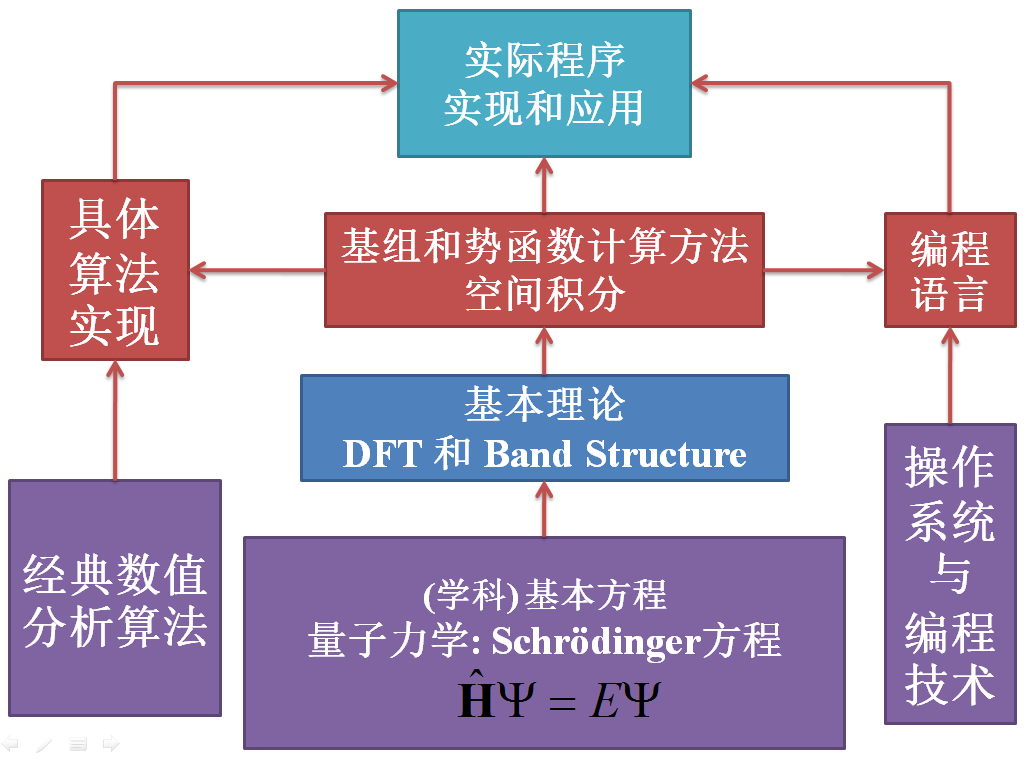
\includegraphics[height=2.80in,width=4.95in,viewport=5 3 1250 780,clip]{Figures/Method_Procedure.png}
%%\caption{\tiny \textrm{Pseudopotential for metallic sodium, based on the empty core model and screened by the Thomas-Fermi dielectric function.}}%(与文献\cite{EPJB33-47_2003}图1对比)
%\label{Method-Procedure}
%\end{figure}
%\end{frame}

\section{计算平台与应用}
\begin{frame}
	\frametitle{适应异质界面催化模拟自动流程软件}
\begin{minipage}[c]{0.42\linewidth}
\begin{itemize}
\vspace*{-2.75in}
%	\item “标准化”对称性分析功能:~降低\textrm{DFT}的计算量
	\item \textcolor{blue}{前处理}:\\
		计算模型分析与预处理
%	\item \textcolor{magenta}{$\vec k\cdot\vec p$方法}:~提升电子计算的规模%,为\textrm{DFT-MD}计算提供基础
	\item \textcolor{blue}{计算流程设计与管理}:\\
		\begin{enumerate}
			\item 支持计算过程的模块化
			\item 支持高通量、跨尺度材料模拟
			\item 提供计算结果数据管理接口
		\end{enumerate}
	\item \textcolor{blue}{后处理}:\\
		结果数据的分析、挖掘与可视化展示
%	\item \textcolor{magenta}{机器学习}:~优化电子计算结果,获得\textrm{MD}尺度力场,\textrm{DFT-MD}耦合%,获得\textrm{MD}尺度下准确的多体相互作用的力场函数。
%	\item 设计合理完善的程序流程:~利用\textrm{MongoDB}支持的\textrm{FireWorks}计算流程管理%,由微观尺度\textrm{DFT}计算获得介观或宏观尺度的计算物性或者使不同尺度的计算结果更好地实现耦合自洽
\end{itemize}
\end{minipage}
\hskip 2pt
\begin{minipage}[b]{0.47\linewidth}
\begin{figure}[h!]
\centering
%\hskip -35pt
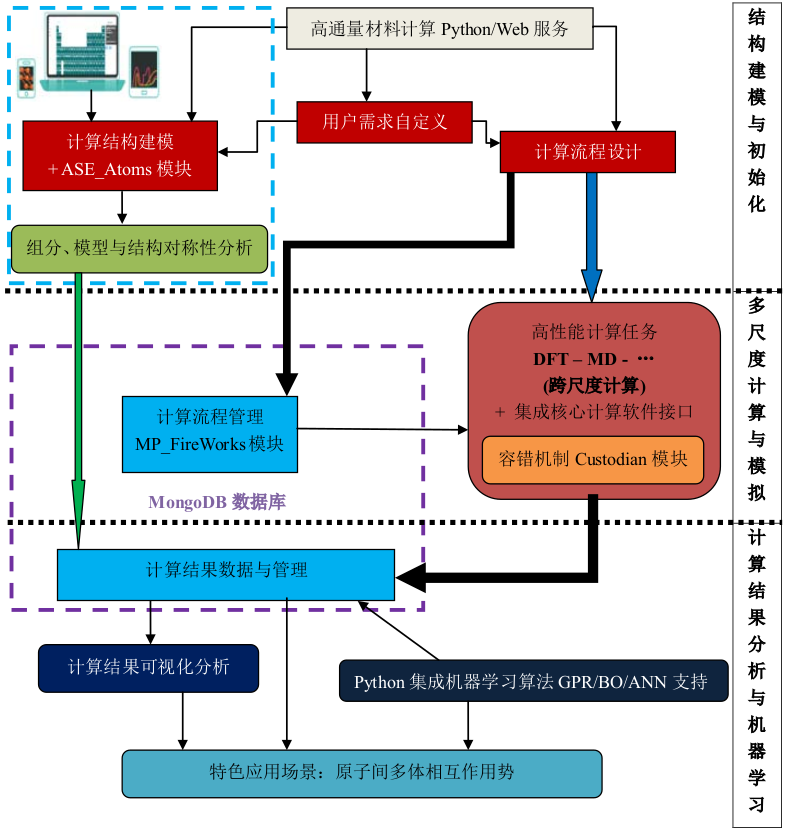
\includegraphics[height=2.18in]{Figures/MP_comp_BCC.png}
\caption{\fontsize{6.5pt}{4.5pt}\selectfont{适用于异质界面的高通量材料计算自动流程软件架构}}%
\label{MP_comp_BCC}
\end{figure}
\end{minipage}
\end{frame}

%\begin{frame}
%	\frametitle{材料智能计算平台}
%	“\textcolor{magenta}{材料多尺度模拟仿真与多目标机器学习大数据平台}”
%	\begin{itemize}
%		\item 材料多尺度模拟流程,电子结构计算优化,化学反应动力学过程与多目标数据收集、特征工程、模型建立和验证等材料机器学习算法相融合
%		\item 材料计算数据库技术应用:~晶体预测结构,半导体带隙,相稳定性,存能与功能材料的物理化学性质等
%	\end{itemize}
%\begin{figure}[h!]
%\centering
%\vspace*{-7pt}
%%\animategraphics[autoplay, loop, width=3.95in, height=1.45in]{15}{Figures/DNN-}{0}{15}
%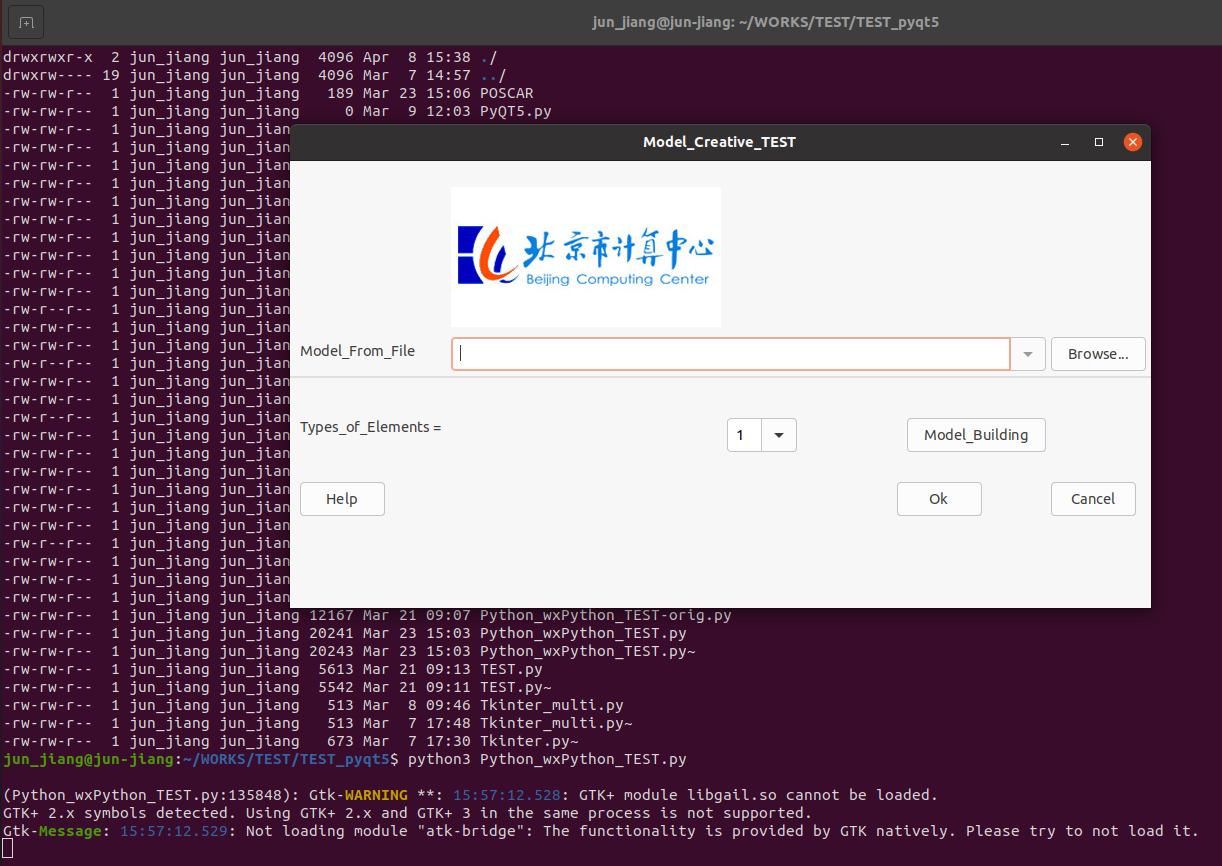
\includegraphics[height=1.60in,width=2.55in,viewport=0 0 1200 870,clip]{Figures/BCC-Process_1.png}
%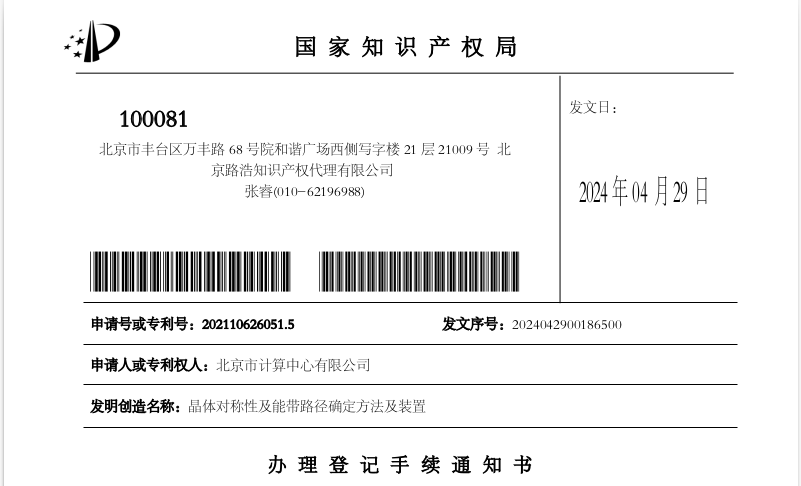
\includegraphics[height=0.85in,width=1.40in,viewport=0 0 801 486,clip]{Figures/Patent_license.png}
%%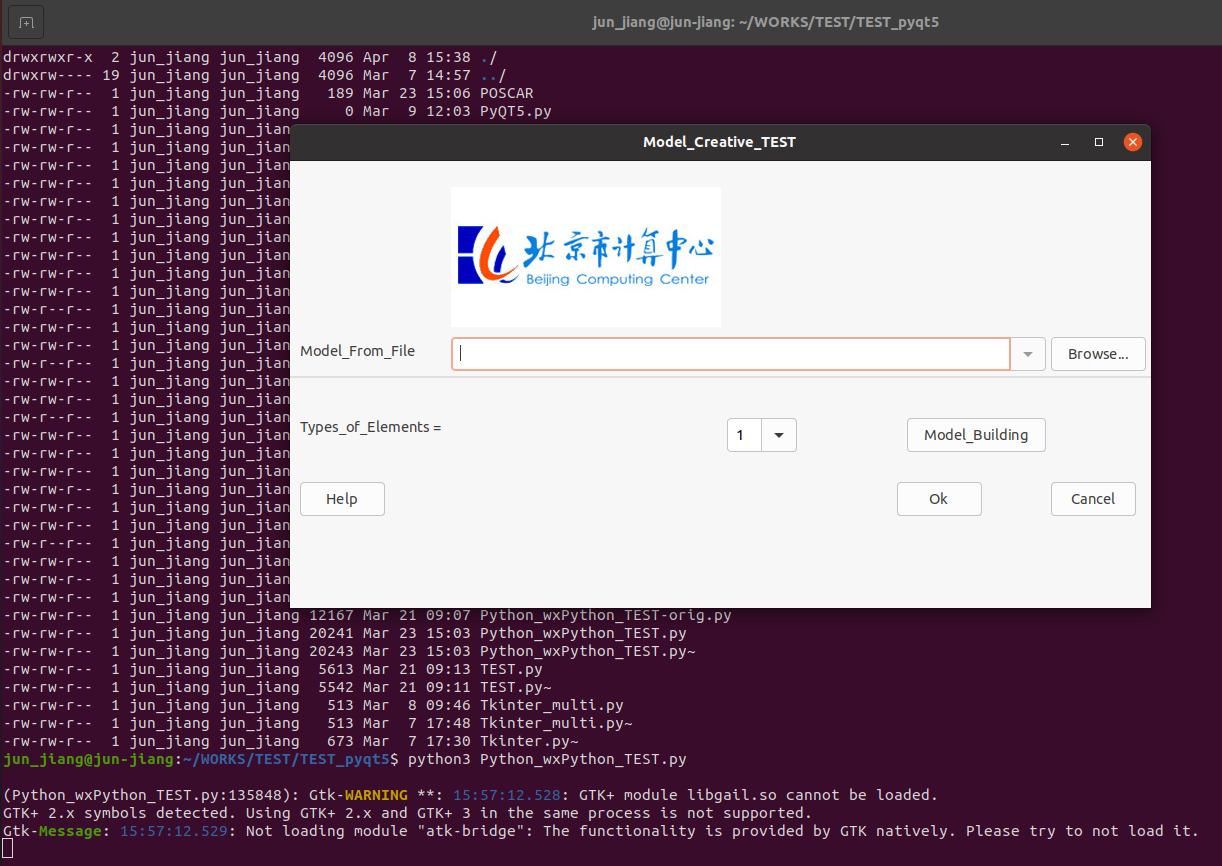
\includegraphics[height=2.00in,width=3.15in,viewport=0 0 1200 870,clip]{Figures/BCC-Process_1.png}
%%\caption{\fontsize{6.5pt}{4.5pt}\selectfont{面向多尺度材料智能计算平台}}%
%\label{BCC-Process_1}
%\end{figure}
%\end{frame}
%
\begin{frame}
	\frametitle{面向多尺度材料智能计算平台}
\begin{figure}[h!]
\centering
%\hskip -35pt
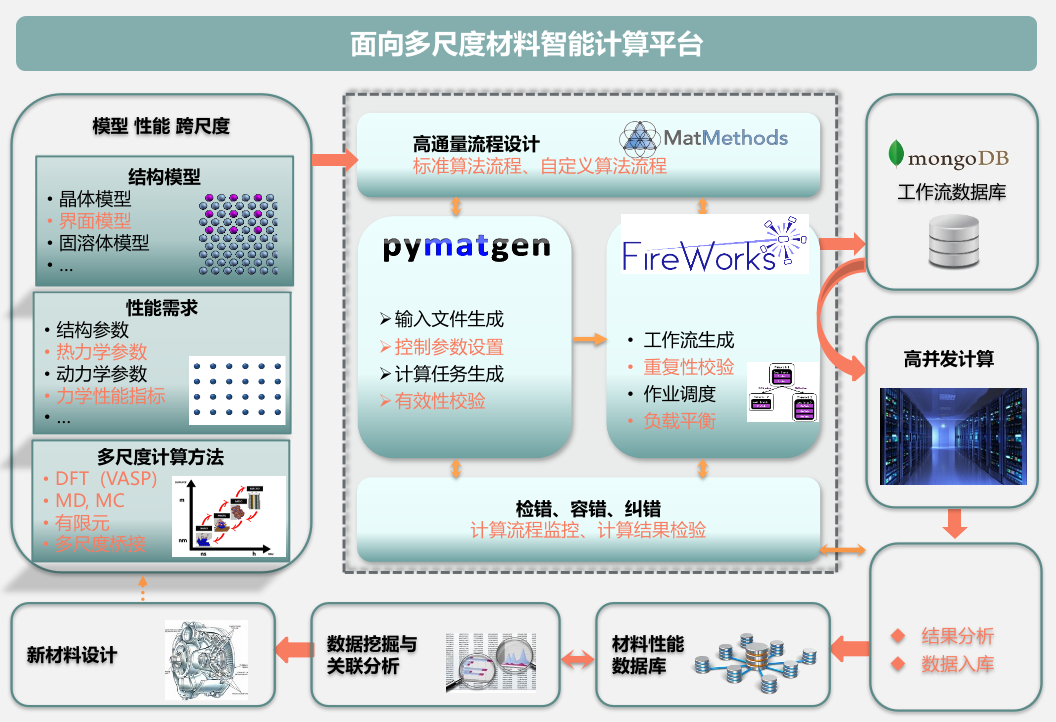
\includegraphics[height=2.75in]{Figures/MP_comp_BCC-2.png}
%\caption{\fontsize{6.5pt}{4.5pt}\selectfont{面向多尺度材料智能计算平台}}%
\label{MP_comp_BCC_2}
\end{figure}
\end{frame}

\begin{frame}
	\frametitle{软硬件全方位集成}
	从自动流程到五阶数据创新材料软硬件一体机
\begin{figure}[h!]
\centering
%\hspace*{-8pt}
\includegraphics[height=1.75in]{Figures/BCC-5-steps_small.jpg}
%\includegraphics[height=1.45in]{Figures/BCC-5-steps.jpg}
%\caption{\fontsize{6.5pt}{4.5pt}\selectfont{面向多尺度材料智能计算平台}}%
\label{BCC-5-steps}
\end{figure}
%{\fontsize{7.5pt}{5.5pt}\selectfont{
\begin{itemize}
	\item 由材料模拟的物理规律转向数据处理能力的提升
	\item 五阶数据处理: 收集、分析、归档、清洗和标准化
	\item 探索数据认知能力,助力材料研究
\end{itemize}
\end{frame}

\begin{frame}
	\frametitle{主要合作与推广}
一体机推广:~提交中科院物理所使用,获得良好反馈
	\begin{itemize}
	 \setlength{\itemsep}{10pt}
		\item 提供的流程软硬件一体机支持凝聚态物理的理论研究
		\item 深化对拓扑绝缘体材料物性特征的认知%,加速对潜在拓扑绝缘体材料的发现
\begin{figure}[h!]
\centering
\vskip 5pt
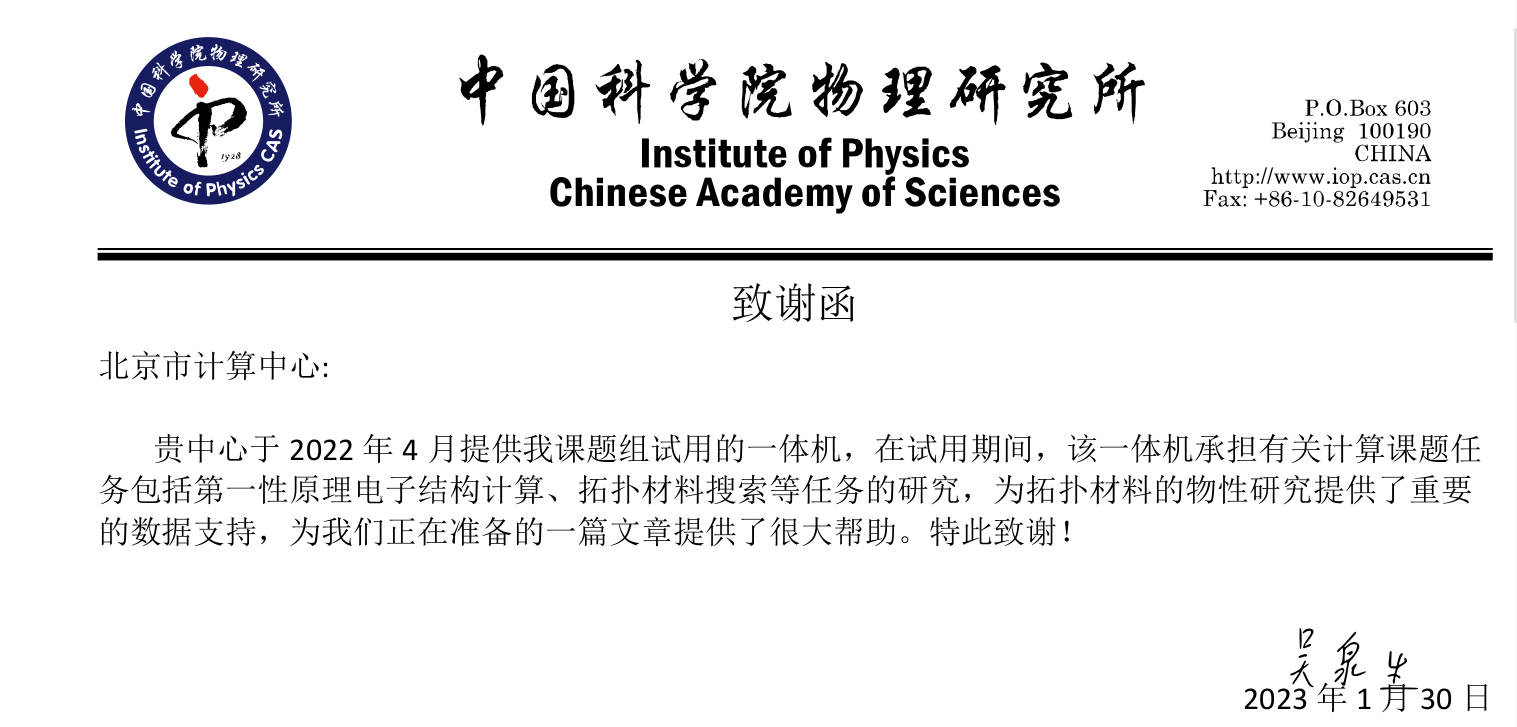
\includegraphics[height=1.7in]{Figures/Acknowledge-IP_CAS-BCC.png}
%\caption{\fontsize{6.5pt}{4.5pt}\selectfont{面向多尺度材料智能计算平台}}%
\label{Acknowleges-IP_CAS}
\end{figure}
	\end{itemize}
\end{frame}

\begin{frame}
	\frametitle{应用:~机器学习构建催化描述符}
\begin{figure}[h!]
\centering
%\hskip -35pt
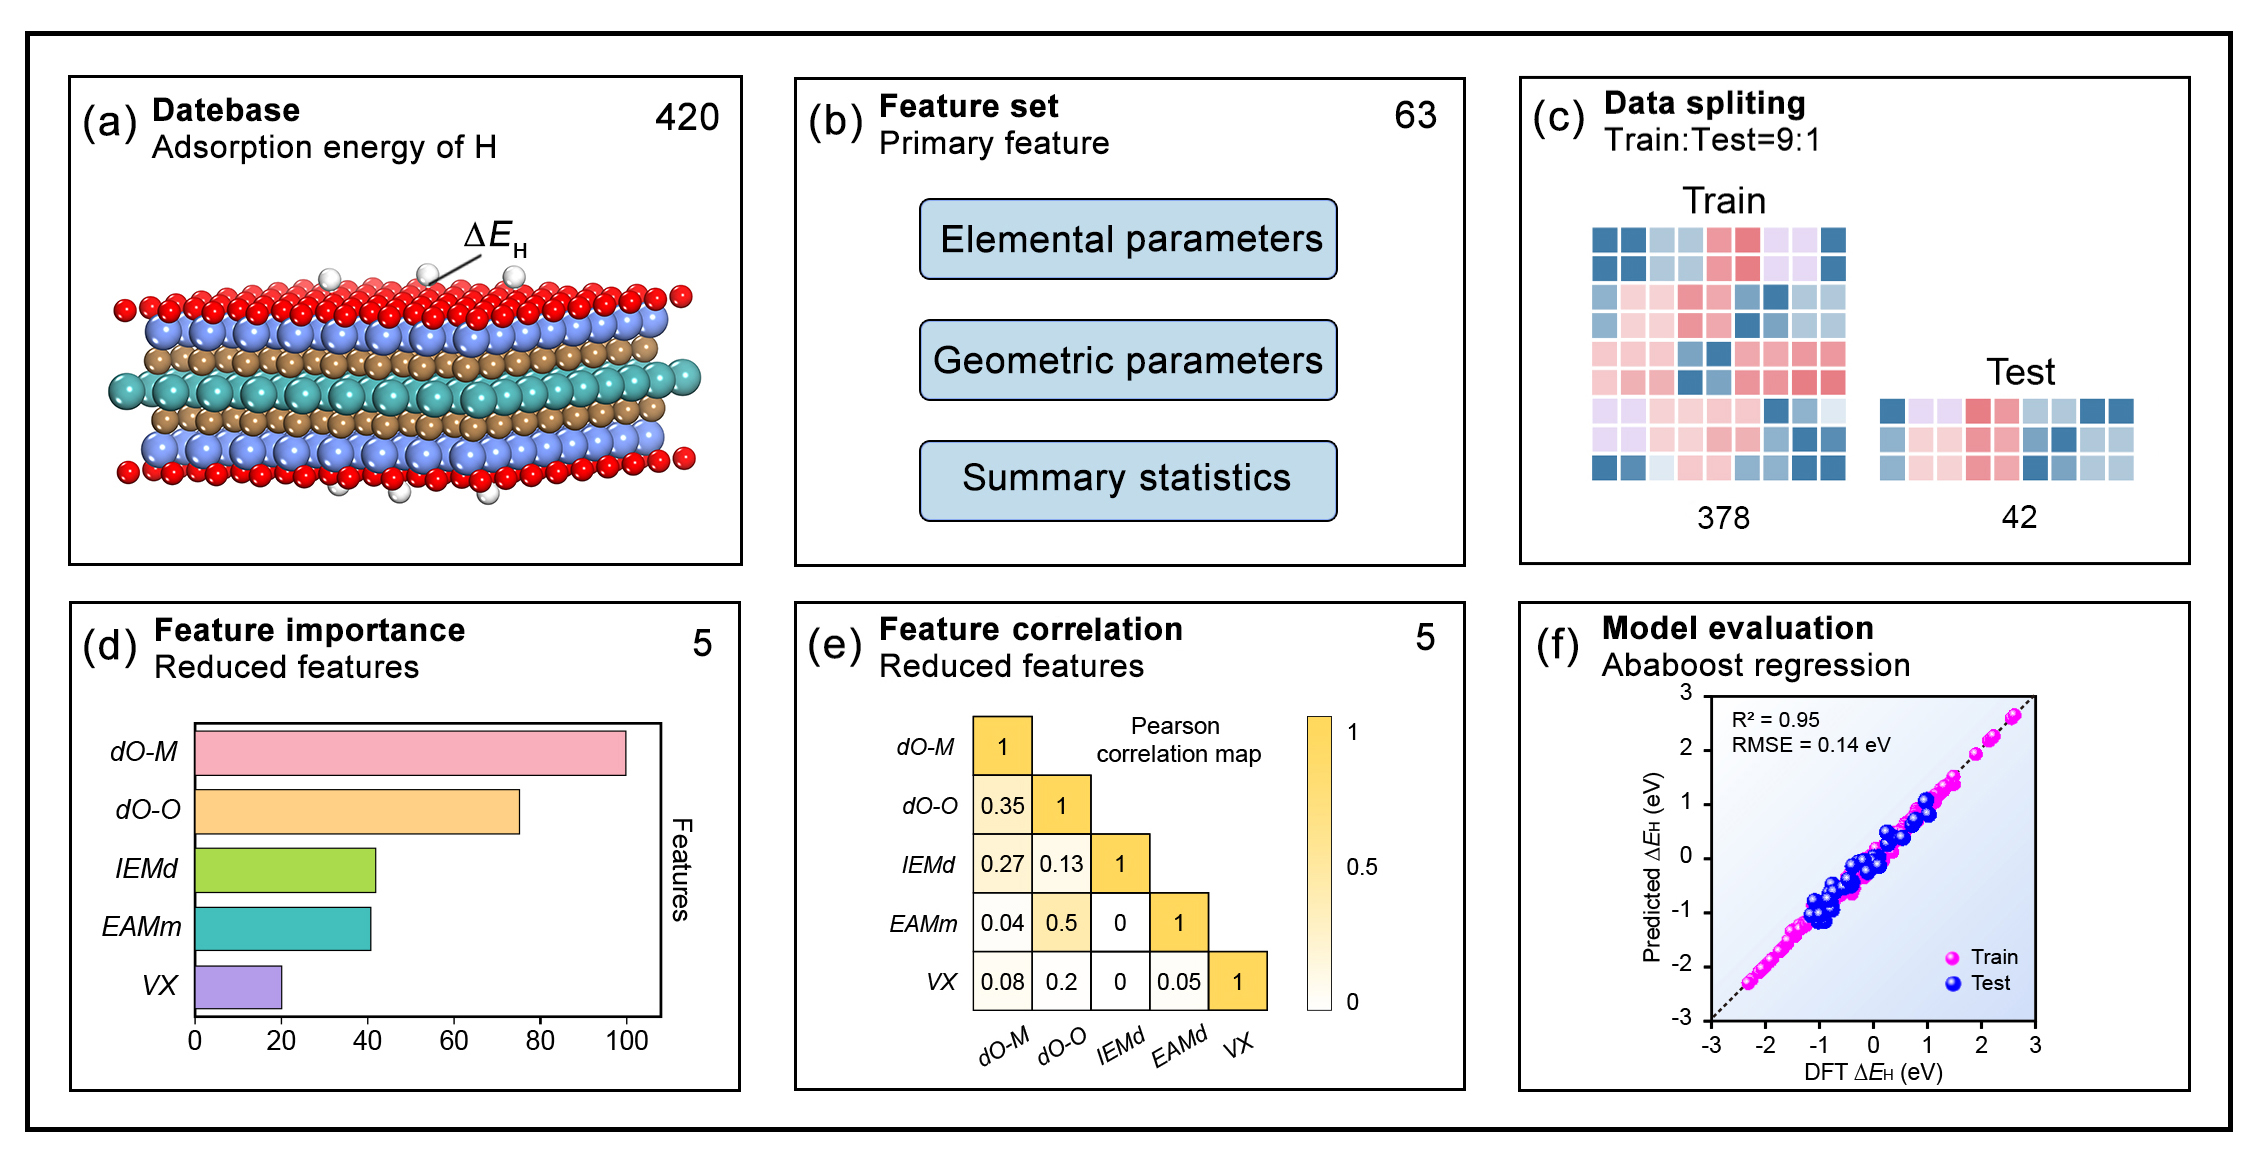
\includegraphics[height=1.85in]{Figures/MP_comp_BCC-4.png}
%\caption{\fontsize{6.5pt}{4.5pt}\selectfont{面向多尺度材料智能计算平台}}%
\label{MP_comp_BCC_4}
\end{figure}
{\fontsize{7.5pt}{5.5pt}\selectfont{
	面向\textrm{2D~MXenes}有序二元合金\textrm{(OBAs)}催化活性:
	\begin{itemize}
		\item 根据理化知识筛选特征向量
		\item 基于机器学习得到好的特征向量
		\item 对多目标优化,检验特征向量间相关度
		\item 基于特征向量筛选潜在优势催化活性材料
	\end{itemize}}}
\end{frame}

\begin{frame}
	\frametitle{应用:~类石墨烯材料产氢性能优化预测}
\begin{figure}[h!]
\centering
%\hskip -35pt
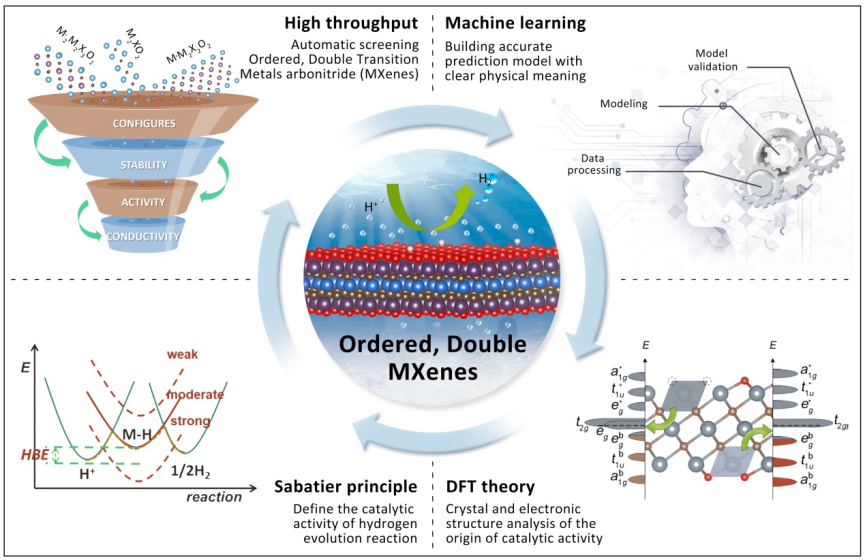
\includegraphics[height=1.85in]{Figures/MP_comp_BCC-3.png}
%\caption{\fontsize{6.5pt}{4.5pt}\selectfont{面向多尺度材料智能计算平台}}%
\label{MP_comp_BCC_3}
\end{figure}
{\fontsize{7.5pt}{5.5pt}\selectfont{
	应用高通量\textrm{DFT}计算,集成机器学习框架,预测\textrm{2D~MXenes}有序二元合金\textrm{(OBAs)}催化活性趋势并指导\textrm{HER}催化剂设计:}}
{\fontsize{5.5pt}{4.5pt}\selectfont{
	\begin{itemize}
		\item 由\textcolor{red}{数千个}\textrm{2D~MXenes}中筛选出的\textcolor{red}{110种}热稳定性、\textrm{HER}活性优于贵金属%\ch{Pt}
		\textrm{Pt}的潜在\textrm{2D~MXenes~OBAs}
	\item 特别是%\ch{Ti}
		\textrm{Ti}元素主要存在于\textrm{2D~MXenes~OBAs}理想催化剂中与实验合成的\textrm{MXenes}一致,\textcolor{red}{提高效率80\%}\\
	\end{itemize}
		获“\textcolor{blue}{2019中国大数据与智能计算技术创新奖}” \\
\textrm{J.~Mater.~Chem.~A,~2020} ~~~~~~~\url{https://doi.org/10.1039/D0TA06583H}}}
\end{frame}

\begin{frame}
	\frametitle{相关成果和奖励}
\begin{figure}[h!]
\centering
\vskip -5pt
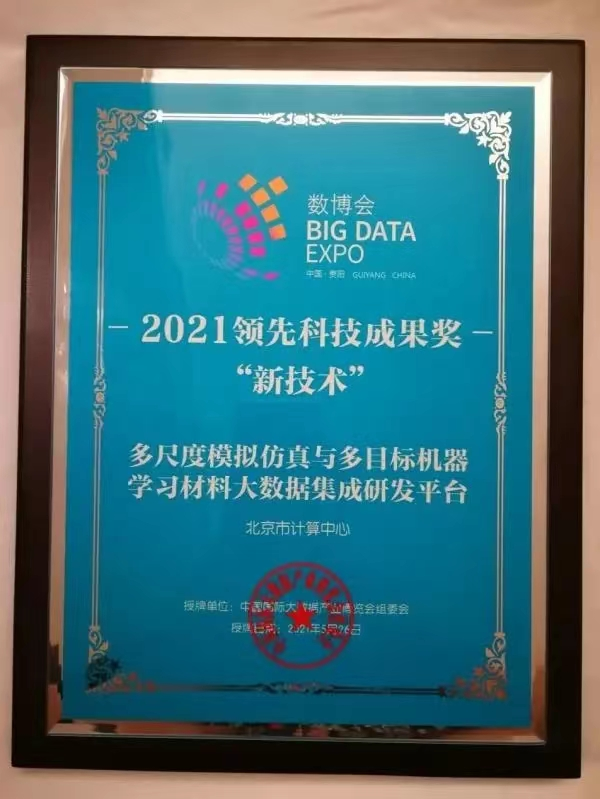
\includegraphics[height=2.5in,width=1.9in]{/home/jun-jiang/BCC/Report_Papers_Awards/2021-BigData_Expo.jpg}
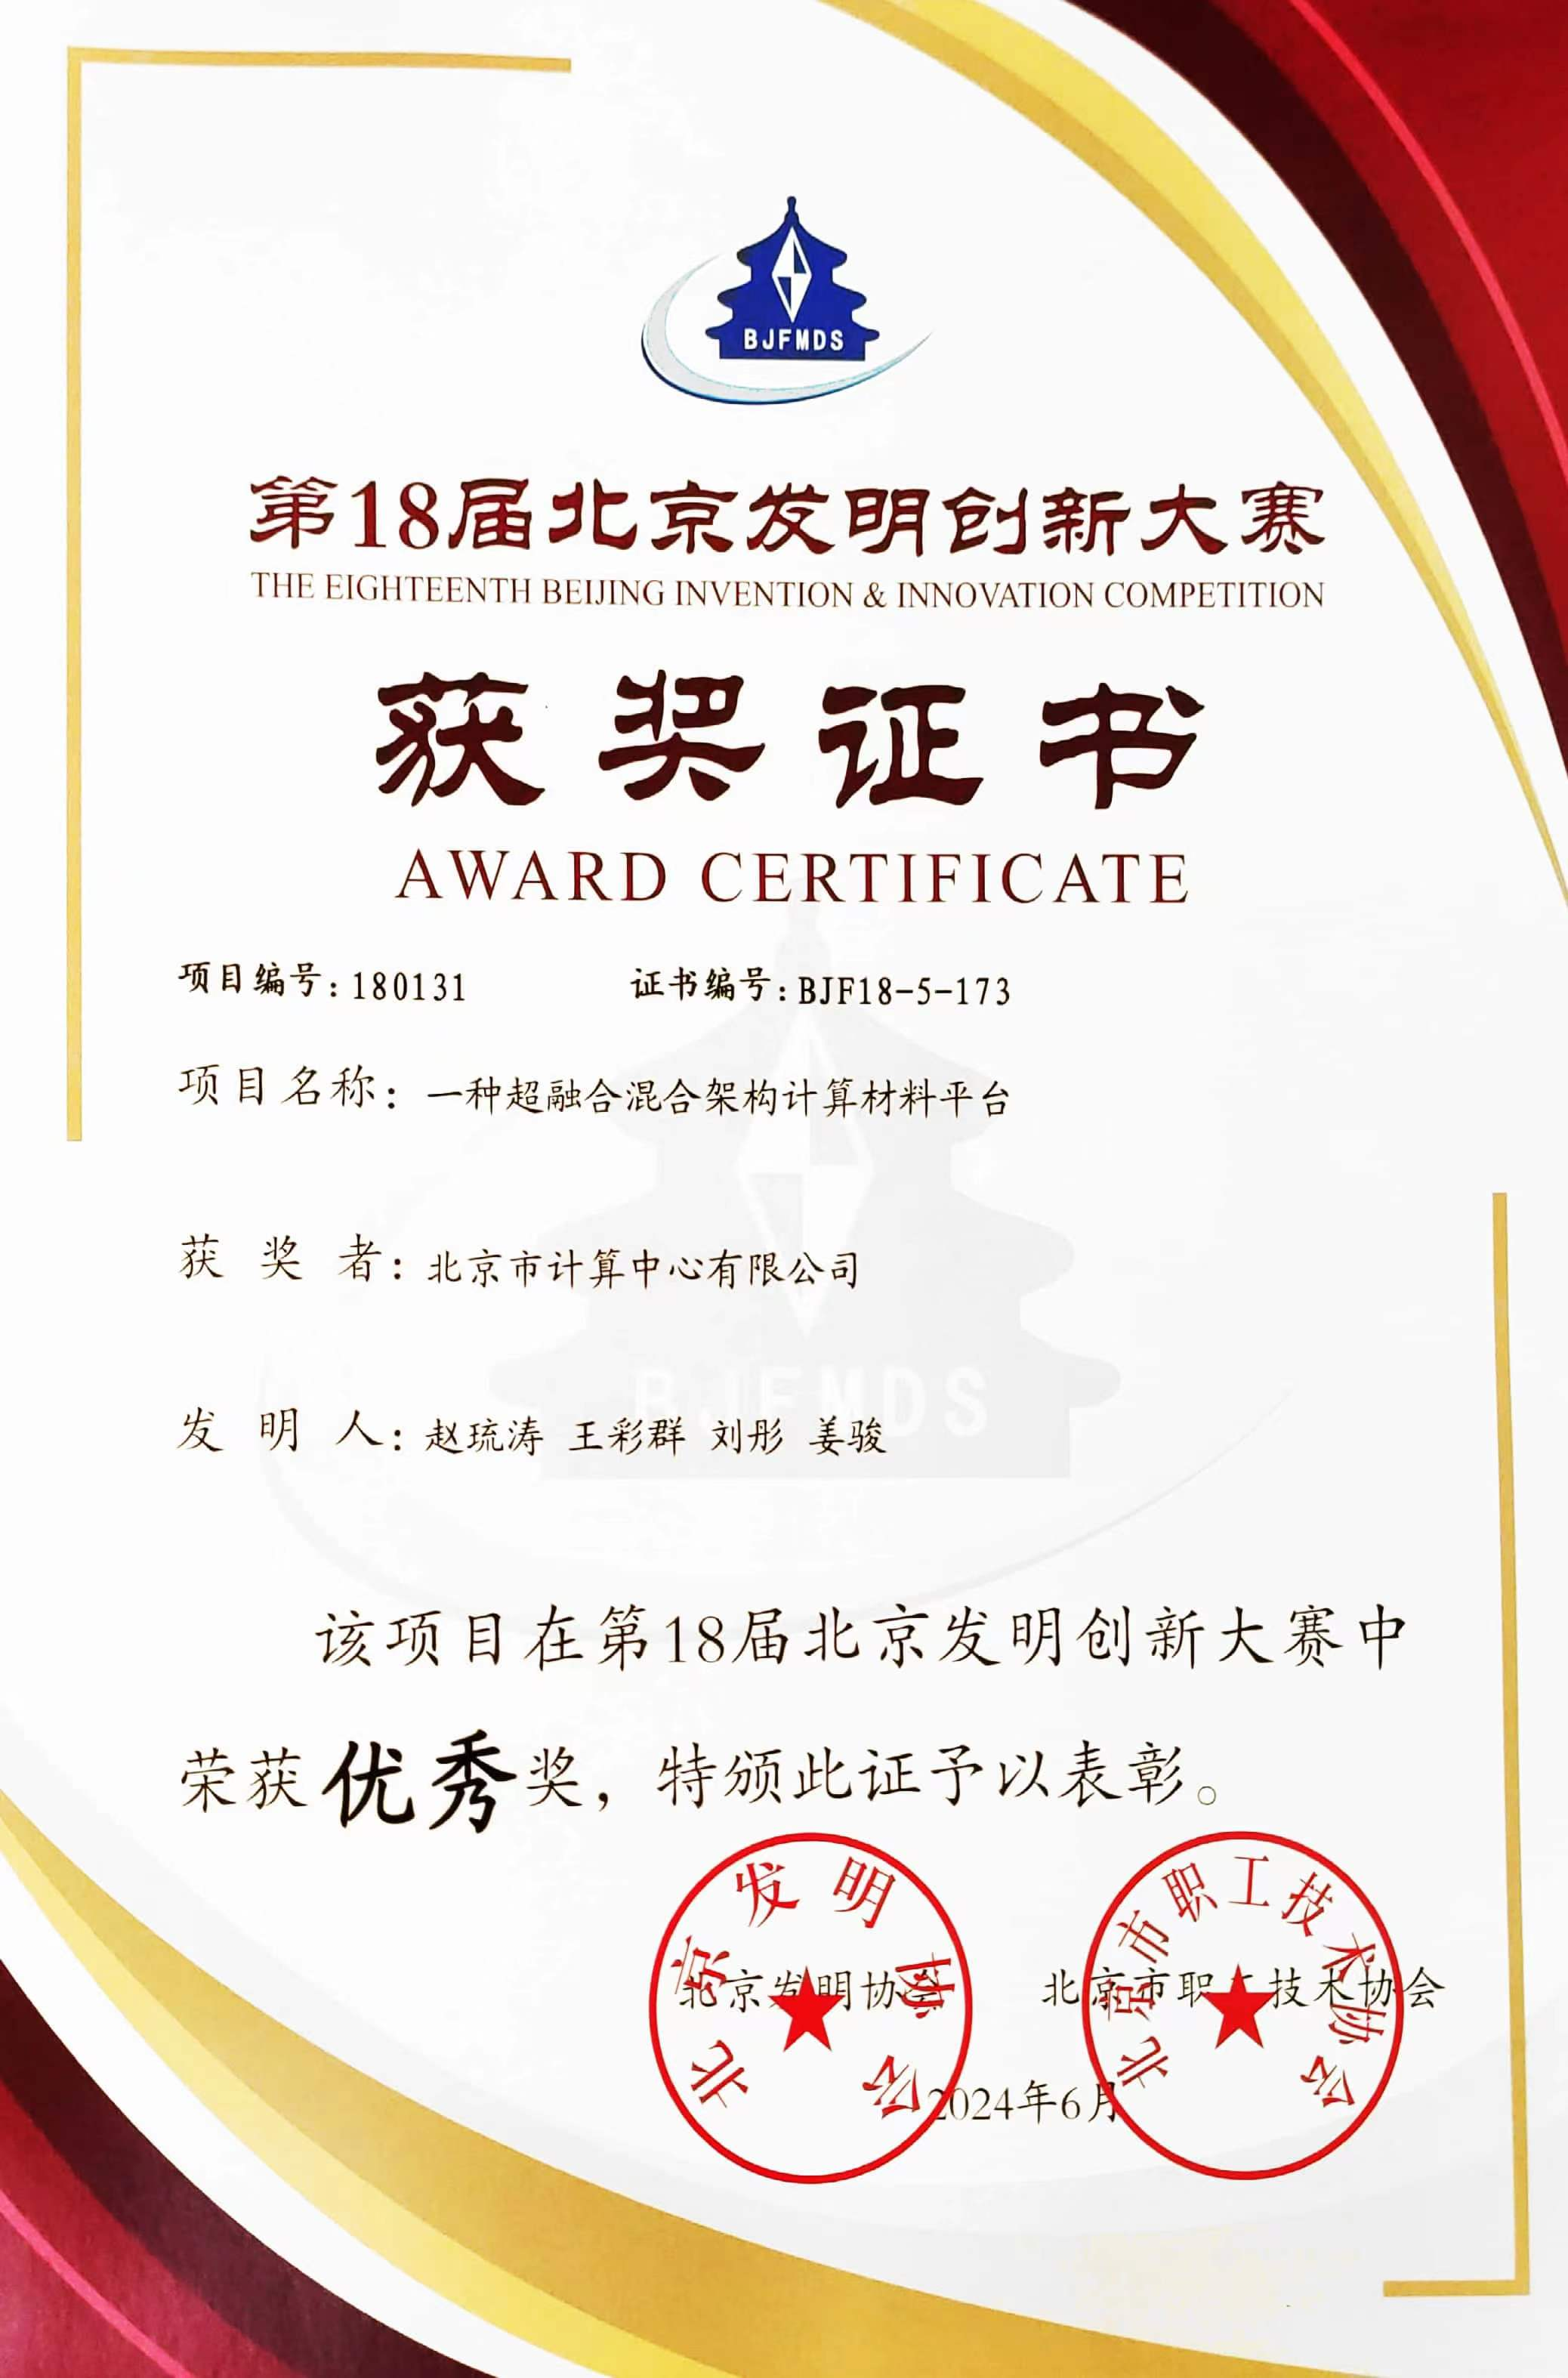
\includegraphics[height=2.5in,width=1.9in]{/home/jun-jiang/BCC/Report_Papers_Awards/2024-Innovation.jpg}
\label{Fig:Award}
%\caption{\fontsize{5.2pt}{6.2pt}\selectfont{$\vec k\cdot\vec p$方法保证计算精度,并计算效率提升}}%
\end{figure}
\end{frame}

\section{材料数据库}
\frame
{
	\frametitle{材料数据积累的相关成果和数据登记}
\begin{figure}[h!]
\vspace*{-0.05in}
\centering
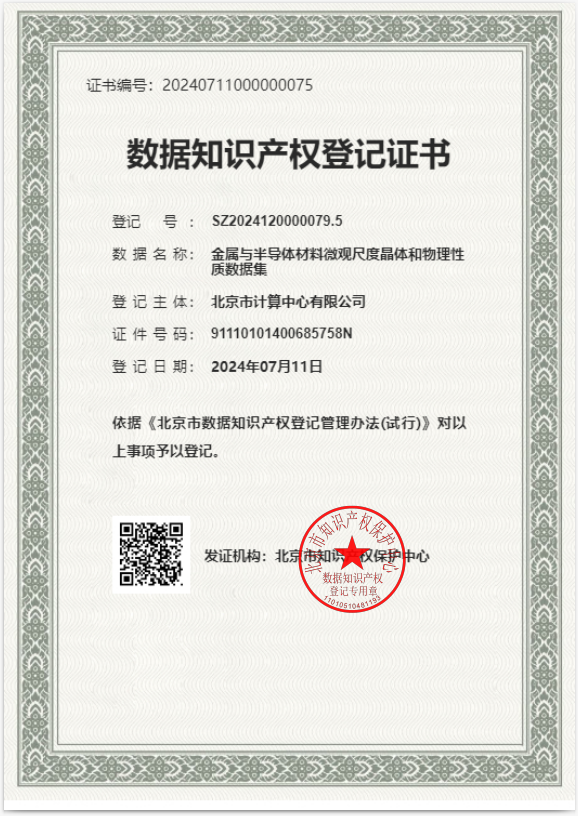
\includegraphics[height=2.75in,width=1.85in,viewport=0 0 579 810,clip]{Figures/Registration_Certificate.png}
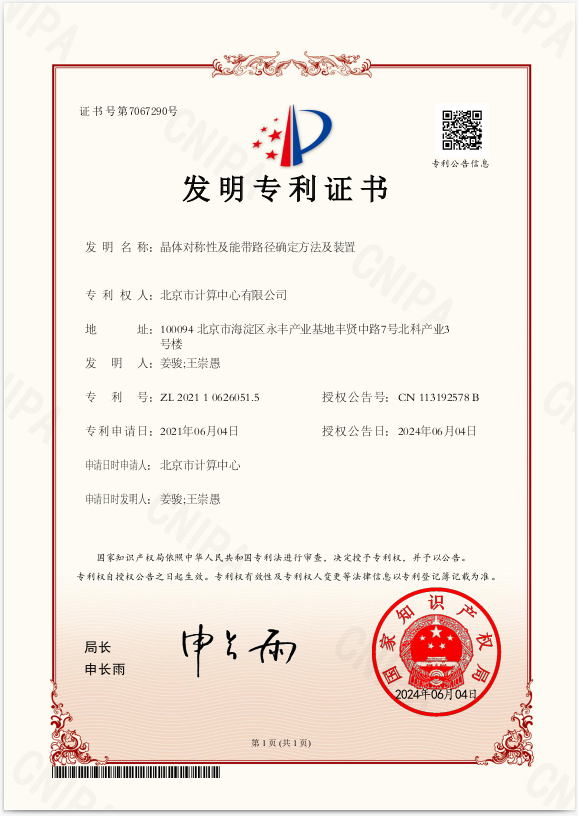
\includegraphics[height=2.75in,width=2.10in,viewport=0 0 609 799,clip]{Figures/Certificate-of-Patent.png}
%\caption{\tiny \textrm{Pseudopotential for metallic sodium, based on the empty core model and screened by the Thomas-Fermi dielectric function.}}%(与文献\cite{EPJB33-47_2003}图1对比)
\label{Certification}
\end{figure}
}

\section{化学-化工知识图谱建设}
\begin{frame}
	\frametitle{化学-化工知识图谱}
	受中科合成油技术股份有限公司委托,开发化学-化工知识图谱,探索\textrm{AI~for~Science}的应用潜力
\begin{figure}[h!]
\centering
%\vskip -8pt
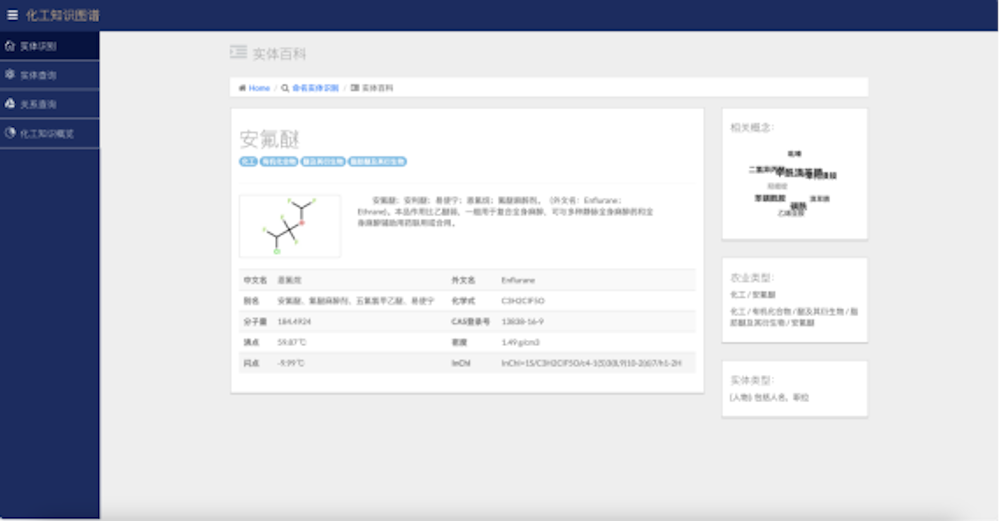
\includegraphics[height=2.20in,width=4.00in,viewport=0 0 240 130,clip]{Figures/KG_Chem-Enflurane.png}
\caption{\tiny 知识图谱的词条内容:~化合物\textrm{安氟醚}的有关知识}%(与文献\cite{EPJB33-47_2003}图1对比)
\label{Fig:KG_Chem-Enflurane}
\end{figure}
\end{frame}

%\begin{frame}
%	\frametitle{应用:~类石墨烯材料的稳定性优化预测}
%\begin{figure}[h!]
%\centering
%%\hskip -35pt
%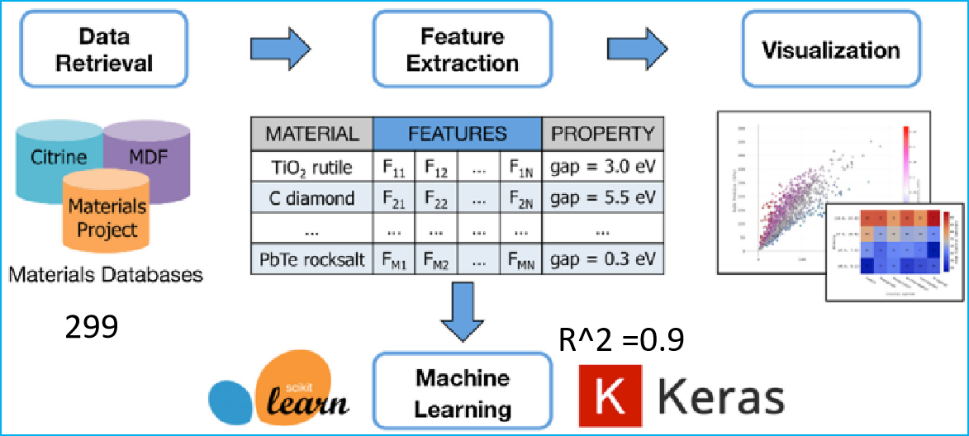
\includegraphics[height=1.55in]{Figures/MP_comp_BCC-5.png}
%%\caption{\fontsize{6.5pt}{4.5pt}\selectfont{面向多尺度材料智能计算平台}}%
%\label{MP_comp_BCC_5}
%\end{figure}
%{\fontsize{7.5pt}{5.5pt}\selectfont{
%	\begin{itemize}
%		\item 应用高通量建模软件构建潜在构型5600多种,利用\textrm{Materials~Projects}材料计算数据库提取竞争相数据
%		\item 通过热分解过程,组合化学反应式2000多组,筛选出热力学稳定的材料299种
%		\item 通过支持向量、高斯过程、随机深林、神经网络以及\textrm{adaboost}多种机器学习回归模型,利用13种常见特征参数对稳定性做了预测
%		\item 预测准确率达到94\%,节省计算成本高达70\%
%	\end{itemize}}}
%\end{frame}
%
%\begin{frame}
%	\frametitle{应用:~监督学习预测半导体材料带隙}
%\begin{figure}[h!]
%\centering
%\hspace*{-8pt}
%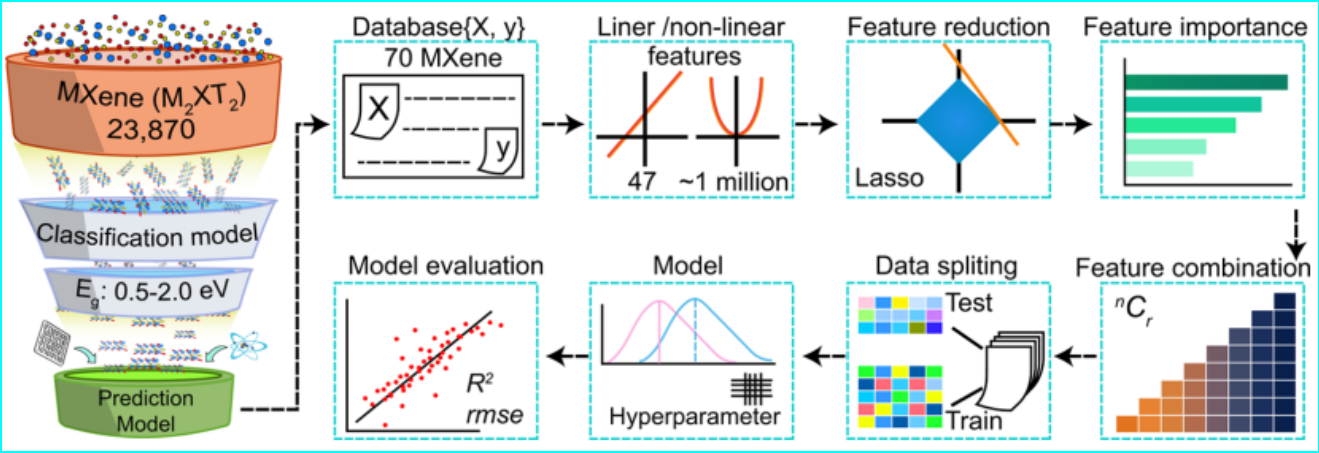
\includegraphics[height=1.45in]{Figures/MP_comp_BCC-6.png}
%%\caption{\fontsize{6.5pt}{4.5pt}\selectfont{面向多尺度材料智能计算平台}}%
%\label{MP_comp_BCC_6}
%\end{figure}
%{\fontsize{7.5pt}{5.5pt}\selectfont{
%	\begin{itemize}
%		\item 常规通行的材料模拟中带隙计算相当耗时
%		\item 利用%类石墨烯新能源
%	材料高通量智能计算与多目标机器学习集成研发平台,高通量自动化快速构建类石墨烯材料结构23870种,并构建数据库结合\textrm{KRR}、\textrm{SVR}、\textrm{GPR}、\textrm{Bagging}机器学习回归模型进行训练预测
%		\item \textrm{GPR}方法预测准确性达到了97\%,可以节省计算成本90\%多
%	\end{itemize}}}
%\end{frame}

\begin{frame}
	\frametitle{化学-化工知识组织的技术实现}
	以知识图谱为例,说明(煤)化学-化工类知识采集、分类与组织
\begin{figure}[h!]
%\vspace*{-0.05in}
\centering
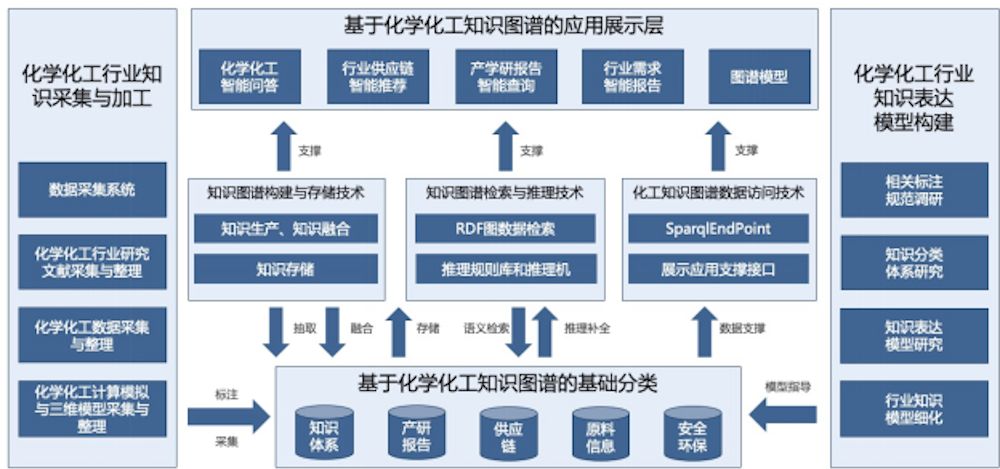
\includegraphics[height=2.08in,width=4.00in,viewport=0 0 245 113,clip]{Figures/KG_Chem-Frame.png}
\caption{\tiny 项目总体技术框架.}%(与文献\cite{EPJB33-47_2003}图1对比)
\label{KG_Chem-Frame}
\end{figure}
\end{frame}

\begin{frame}
	\frametitle{数据:~一切知识的基础}
\begin{figure}[h!]
\centering
\vskip -8pt
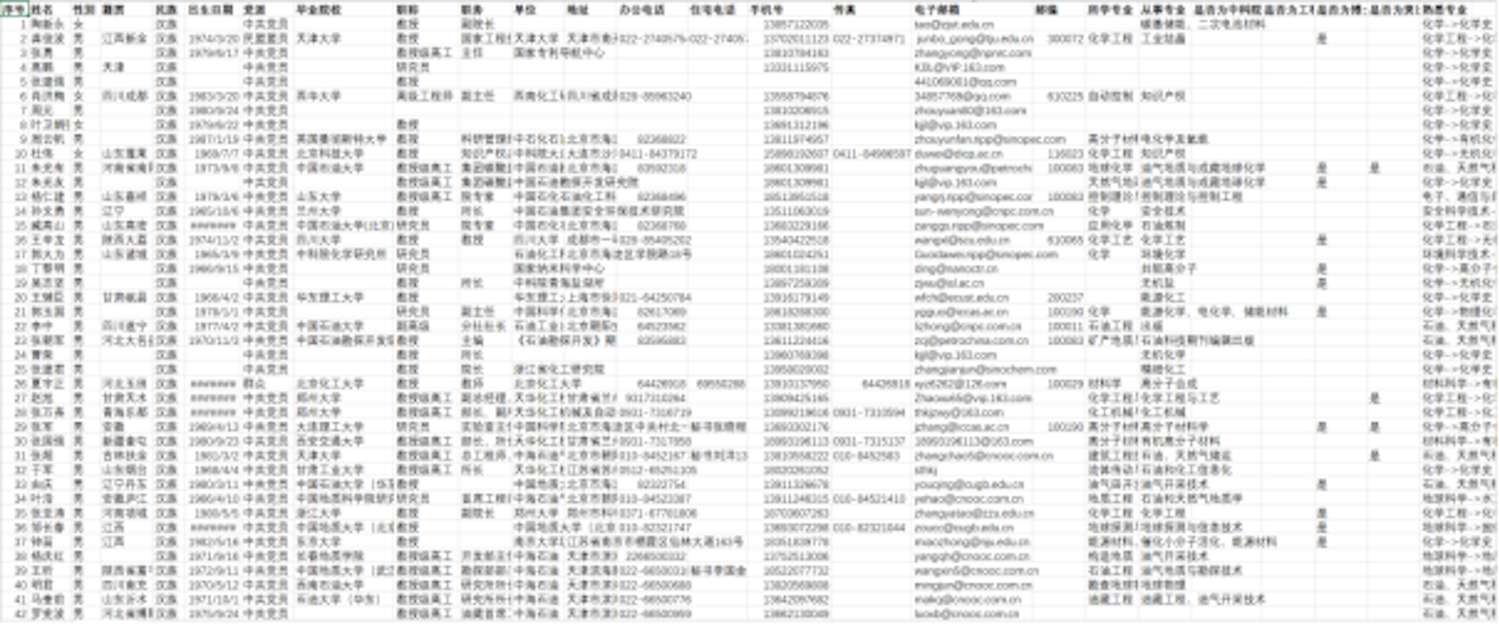
\includegraphics[height=2.10in,width=4.00in,viewport=0 0 210 95,clip]{Figures/KG_Chem-Info.png}
\caption{\tiny 有组织的数据是一切\textrm{AI}知识的基础}%(与文献\cite{EPJB33-47_2003}图1对比)
\label{Fig:KG_Chem-Enflurane}
\end{figure}
\end{frame}

\begin{frame}
	\frametitle{数据的提取}
\begin{figure}[h!]
\centering
%\vskip -8pt
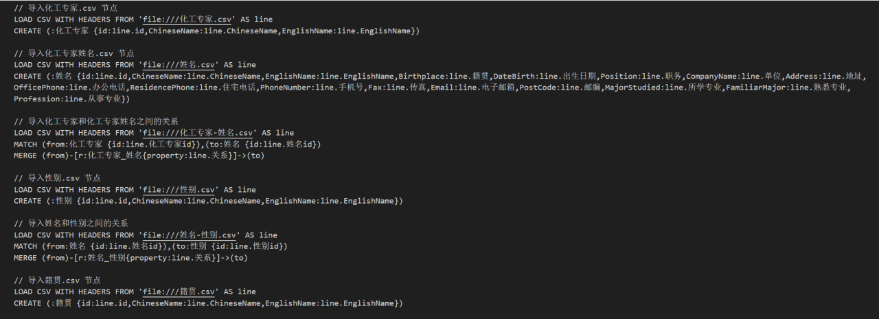
\includegraphics[height=1.60in,width=4.00in,viewport=0 0 210 80,clip]{Figures/KG_Chem-extract.png}
\caption{\tiny 数据的提取是一切\textrm{AI}知识分类的逻辑起点}%(与文献\cite{EPJB33-47_2003}图1对比)
\label{Fig:KG_Chem-Extract}
\end{figure}
\end{frame}

\begin{frame}
	\frametitle{知识图谱\textrm{RDF}图数据检索}
\begin{figure}[h!]
\centering
%\vskip -8pt
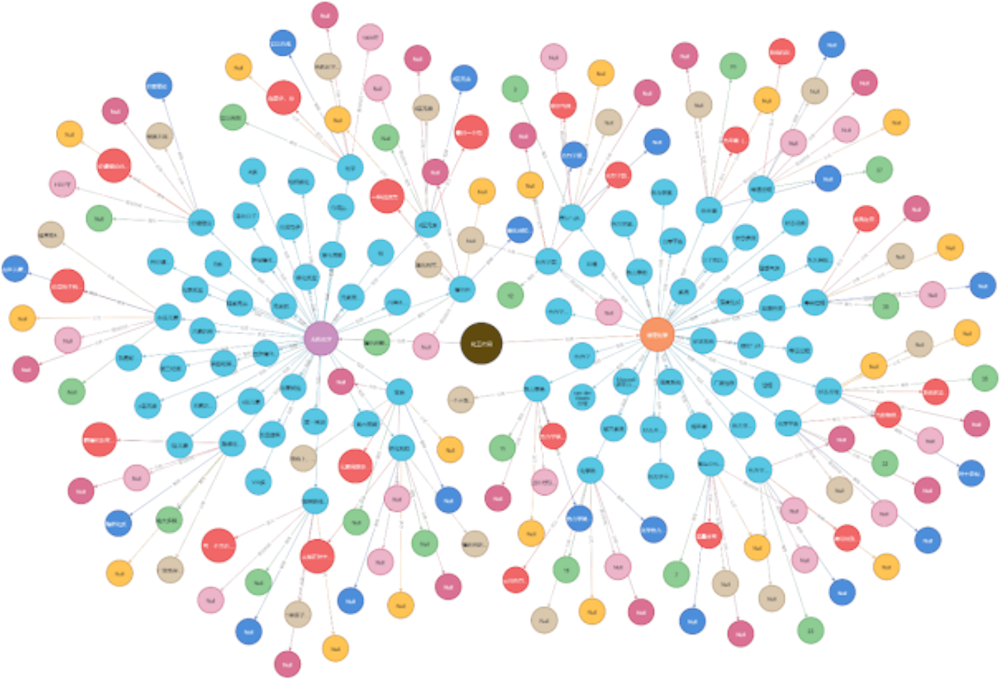
\includegraphics[height=2.60in,width=4.00in,viewport=0 0 240 180,clip]{Figures/KG_Chem-Inorganic.png}
\caption{\tiny 知识图谱的数据\textrm{RDF}图:~无机化合物}%(与文献\cite{EPJB33-47_2003}图1对比)
\label{Fig:KG_Chem-Inorganic}
\end{figure}
\end{frame}

\begin{frame}
	\frametitle{化学-化工知识图谱:~示例}
\begin{figure}[h!]
\centering
%\vskip -8pt
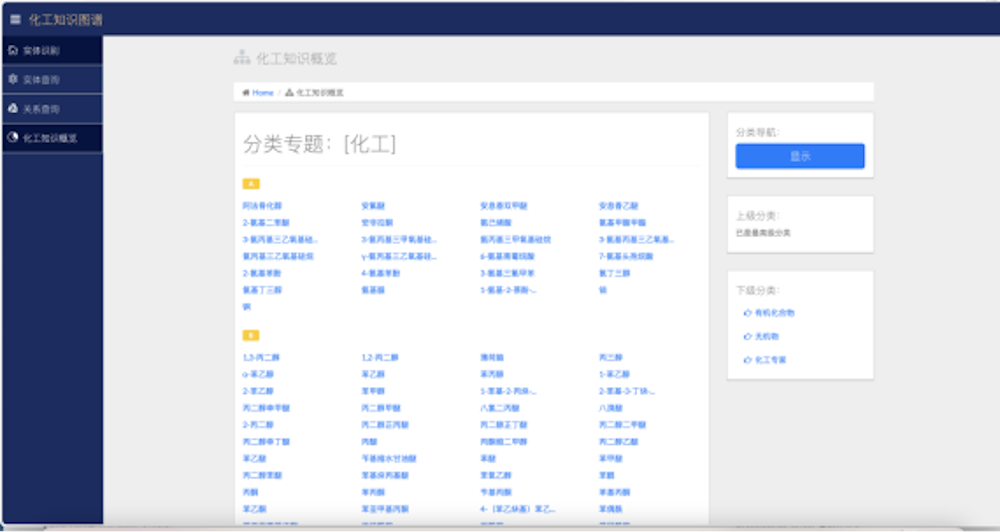
\includegraphics[height=2.10in,width=4.00in,viewport=0 0 240 130,clip]{Figures/KG_Chem-html.png}
\caption{\tiny 化学-化工知识图谱网页}%(与文献\cite{EPJB33-47_2003}图1对比)
\label{Fig:KG_Chem-Enflurane}
\end{figure}
\end{frame}

%\frame
%{
%	\frametitle{化学-化工知识图谱的组成}
%\begin{figure}[h!]
%\centering
%\vskip -8pt
%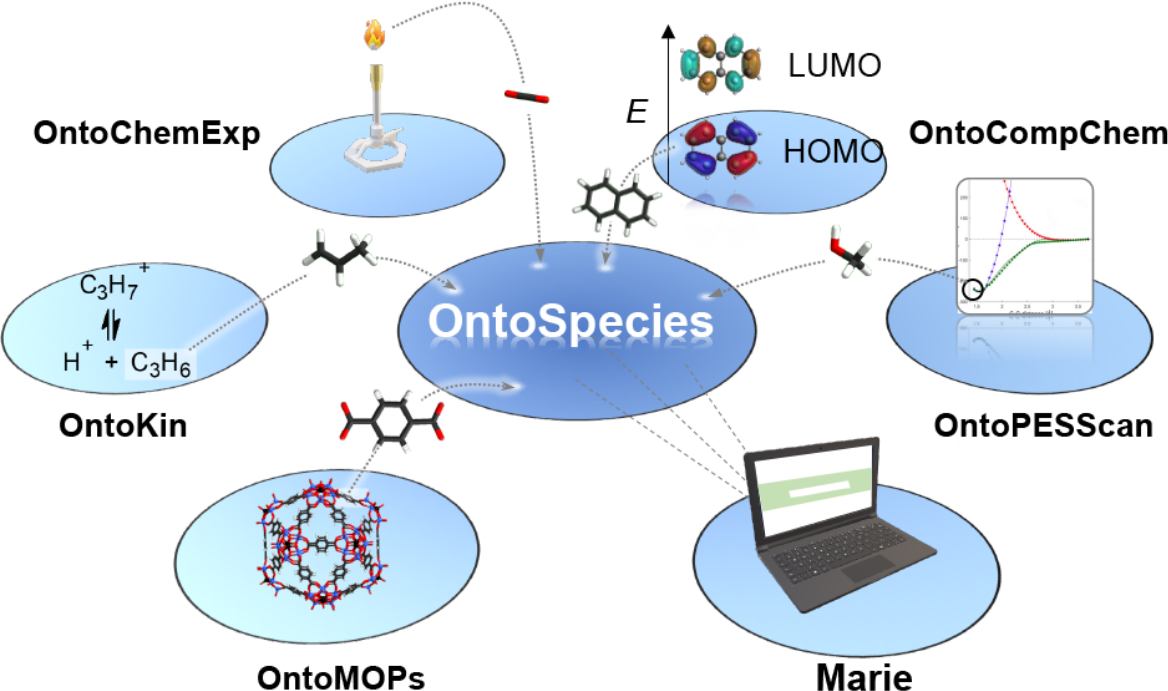
\includegraphics[height=2.45in,width=4.05in,viewport=0 0 1170 700,clip]{Figures/Connection-of-OntoSpecies-to-segments-of-KG.png}
%\caption{\tiny\textrm{Connection of OntoSpecies to other segments of TWA KG. cite from~\cite{ACR56-128_2023}}}%(与文献\cite{EPJB33-47_2003}图1对比)
%\label{Fig:OntoSpecies-to-segments-TWA}
%\end{figure}
%}
%
%\frame
%{
%	\frametitle{化学-化工知识图谱}
%	化学-化工知识图谱:~以化学物种(元素、化合物)为核心的\textcolor{cyan}{多个知识的\textrm{Ontology}组成}
%	\begin{itemize}
%		\item \textrm{OntoSpecites}:~主要纪录化学物种的知识,包括分子式、电荷、分子量和自旋多重度等
%		\item \textrm{OntoKin}:~表示反应机理的知识,纪录反应物、产物和反应过程的信息
%		\item \textrm{OntoCompChem}:~表示计算化学的信息的知识,计算信息的描述包括
%			\begin{itemize}
%				\item 计算对象:~单点计算、结构优化和频率计算
%				\item 计算使用的软件,{\fontsize{7.2pt}{5.2pt}\selectfont{如\textrm{Gaussian~16}}}
%				\item 计算中使用的方法,包括泛函和基组{\fontsize{7.2pt}{5.2pt}\selectfont{~如\textrm{B3LYP,~6-31G(d)}}}
%				\item 电荷与自旋极化
%			\end{itemize}
%		\item \textrm{OntoCompExp}:~表示化学实验信息的知识,包括各类化学实验条件
%	\end{itemize}
%}
%
%\frame
%{
%	\frametitle{\textrm{OntoSpecies}:~化学物种的描述}
%\begin{figure}[h!]
%\centering
%\vskip -8pt
%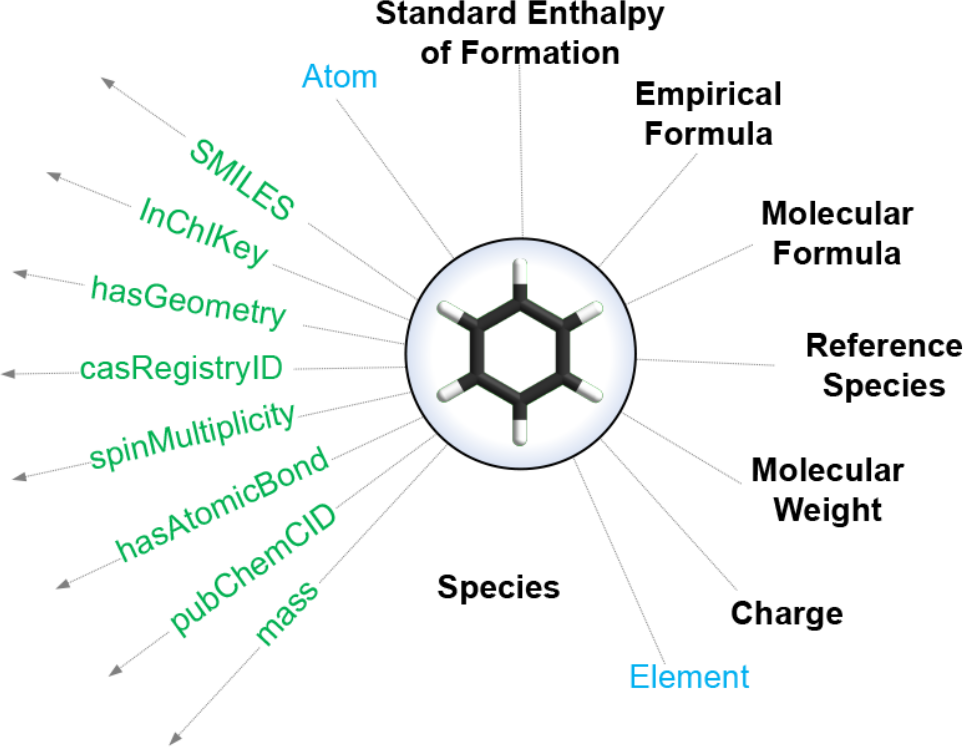
\includegraphics[height=2.40in,width=3.25in,viewport=0 0 990 750,clip]{Figures/Key_OntoSpecies-and-external_concepts.png}
%\caption{\tiny\textrm{Key OntoSpecies (black) and external (blue) concepts, along with a number of properties (green) used to describe chemical species in TWA KG. cite from~\cite{ACR56-128_2023}}}%(与文献\cite{EPJB33-47_2003}图1对比)
%\label{Fig:Key-OntoSpecies-and-external-concepts}
%\end{figure}
%}
%
%\frame
%{
%	\frametitle{\textrm{Agent}:~化学-化工知识图谱的组织工具}
%	\textrm{Agent}:~能够感知环境、进行决策和执行动作的智能处理软件
%	\begin{itemize}
%		\item \textrm{Agent}工作方式类似于人类代理:~能接收输入数据(如传感器信息、文本、图像等),通过分析和处理数据,理解环境和任务要求,并做出相应的决策和行动
%		\item 应用场景广泛,如自动驾驶车辆、智能机器人、语音助手等
%		\item \textrm{Agent}核心功能:~感知、推理和决策
%			\begin{itemize}
%				\item 感知:~通过传感器等方式获取环境信息的能力,例如通过摄像头获取图像或通过麦克风获取声音
%				\item 推理:~基于获取的信息进行逻辑推理和分析的能力,以了解环境和任务需求
%				\item 决策:~根据推理结果做出相应的决策,并执行相应的动作
%			\end{itemize}
%		\item 通过与环境的交互和反馈,\textrm{Agent}可以逐步改进性能和表现,实现好的任务执行能力\\
%		\item \textrm{Agent}设计和训练,需要结合机器学习和人工智能技术,如强化学习、深度学习等
%	\end{itemize}
%}
%
%\frame
%{
%	\frametitle{知识图谱组织示例}
%\begin{figure}[h!]
%\centering
%\vskip -8pt
%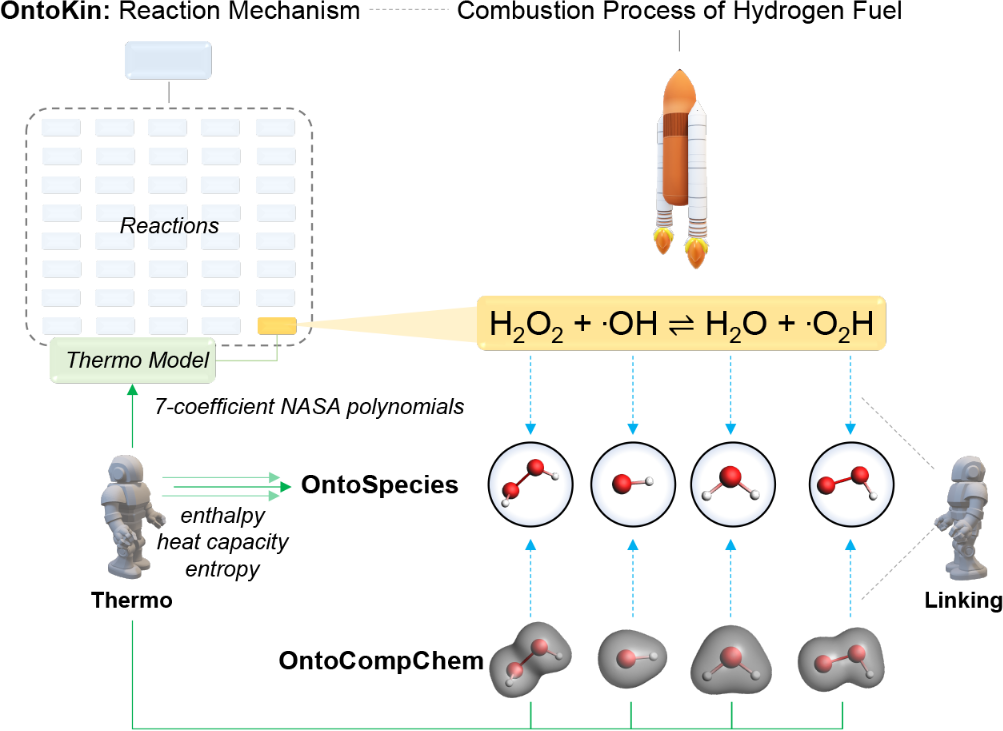
\includegraphics[height=2.70in,width=3.75in,viewport=0 0 1010 750,clip]{Figures/Automated-linking-between-OntoSepcies-Kin-CompChem.png}
%\caption{\tiny\textrm{Automated linking between OntoSpecies, OntoKin and OntoCompChem. cite from~\cite{ACR56-128_2023}}}%(与文献\cite{EPJB33-47_2003}图1对比)
%\label{Fig:Automated-linking-between-OntoSpecies-Kin-CompChem}
%\end{figure}
%}
%
%\frame
%{
%	\frametitle{知识图谱组织示例}
%\begin{figure}[h!]
%\centering
%\vskip -8pt
%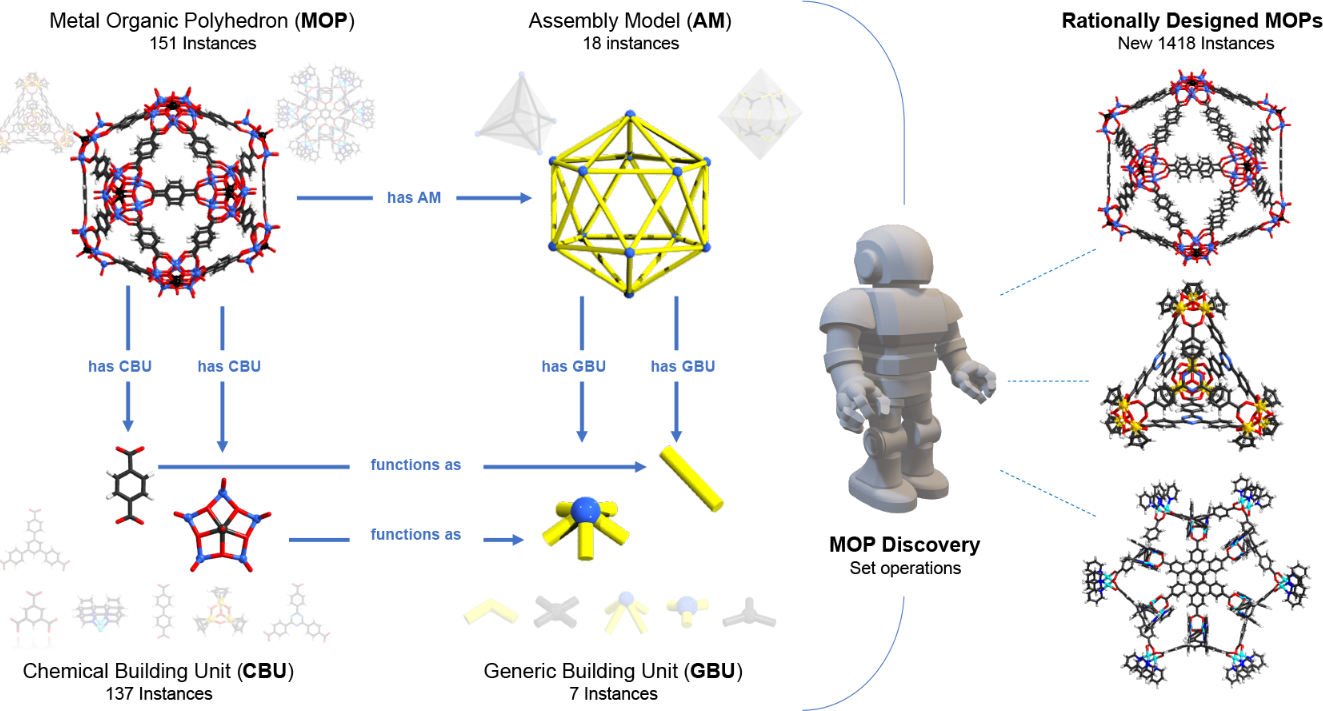
\includegraphics[height=2.20in,width=4.05in,viewport=0 0 1330 700,clip]{Figures/Key_concepts-in-OntoMOPs-and-designed-MOPs.png}
%\caption{\tiny\textrm{Key concepts in OntoMOPs (left) and examples of newly rationally designed MOPs (right). cite from~\cite{ACR56-128_2023}}}%(与文献\cite{EPJB33-47_2003}图1对比)
%\label{Fig:OntoMOPs-MOPs}
%\end{figure}
%}

%\begin{frame}
%	\frametitle{应用:~类石墨烯材料的稳定性优化预测}
%\begin{figure}[h!]
%\centering
%%\hskip -35pt
%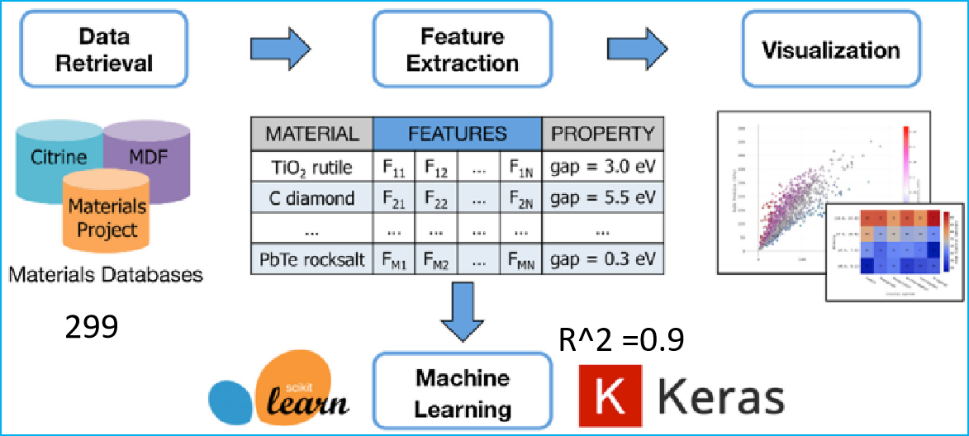
\includegraphics[height=1.55in]{Figures/MP_comp_BCC-5.png}
%%\caption{\fontsize{6.5pt}{4.5pt}\selectfont{面向多尺度材料智能计算平台}}%
%\label{MP_comp_BCC_5}
%\end{figure}
%{\fontsize{7.5pt}{5.5pt}\selectfont{
%	\begin{itemize}
%		\item 应用高通量建模软件构建潜在构型5600多种,利用\textrm{Materials~Projects}材料计算数据库提取竞争相数据
%		\item 通过热分解过程,组合化学反应式2000多组,筛选出热力学稳定的材料299种
%		\item 通过支持向量、高斯过程、随机深林、神经网络以及\textrm{adaboost}多种机器学习回归模型,利用13种常见特征参数对稳定性做了预测
%		\item 预测准确率达到94\%,节省计算成本高达70\%
%	\end{itemize}}}
%\end{frame}
%
%\begin{frame}
%	\frametitle{应用:~监督学习预测半导体材料带隙}
%\begin{figure}[h!]
%\centering
%\hspace*{-8pt}
%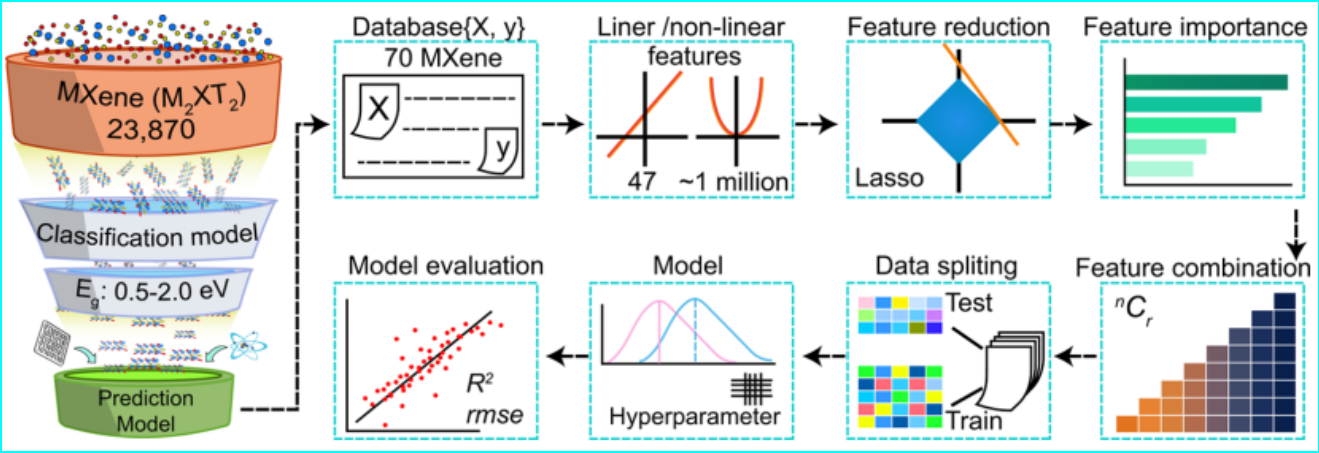
\includegraphics[height=1.45in]{Figures/MP_comp_BCC-6.png}
%%\caption{\fontsize{6.5pt}{4.5pt}\selectfont{面向多尺度材料智能计算平台}}%
%\label{MP_comp_BCC_6}
%\end{figure}
%{\fontsize{7.5pt}{5.5pt}\selectfont{
%	\begin{itemize}
%		\item 常规通行的材料模拟中带隙计算相当耗时
%		\item 利用%类石墨烯新能源
%	材料高通量智能计算与多目标机器学习集成研发平台,高通量自动化快速构建类石墨烯材料结构23870种,并构建数据库结合\textrm{KRR}、\textrm{SVR}、\textrm{GPR}、\textrm{Bagging}机器学习回归模型进行训练预测
%		\item \textrm{GPR}方法预测准确性达到了97\%,可以节省计算成本90\%多
%	\end{itemize}}}
%\end{frame}

%\begin{frame}[allowframebreaks]
%	\frametitle{主要合作与推广应用}
%		中科合成油(合作)
%	\begin{itemize}
%	 \setlength{\itemsep}{30pt}
%	\item 化学-化工知识图谱的建设
%\begin{figure}[h!]
%\centering
%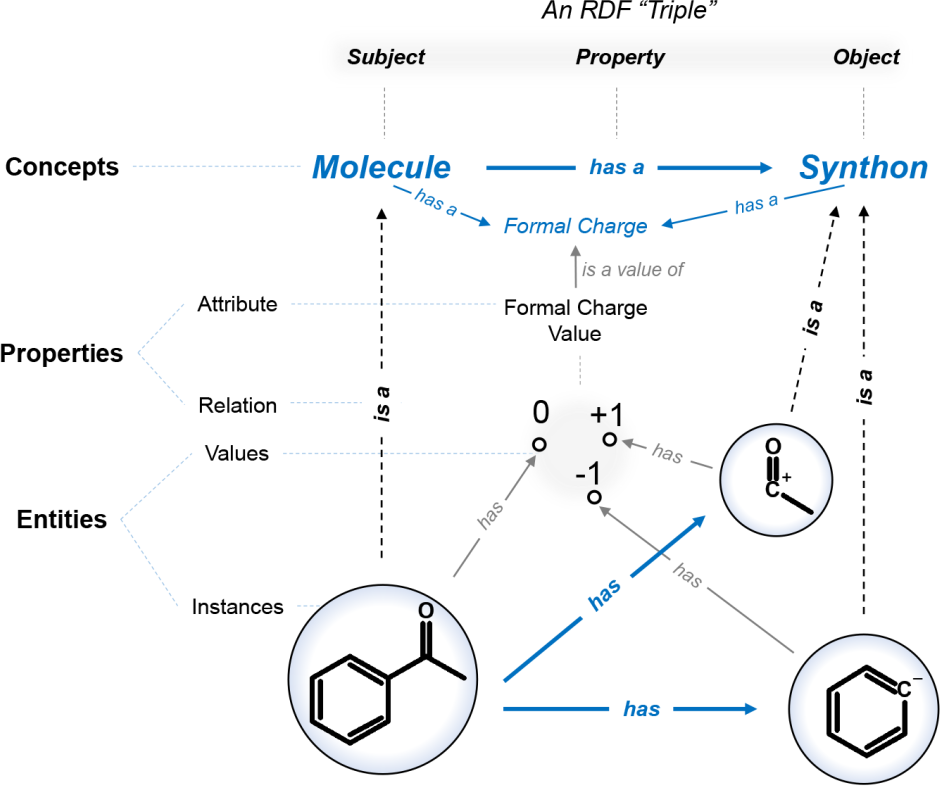
\includegraphics[height=1.50in,width=1.75in,viewport=0 0 950 790,clip]{Figures/Mapping-the-relationship-between-molecule-and-synthon.png}
%\hspace{5pt}
%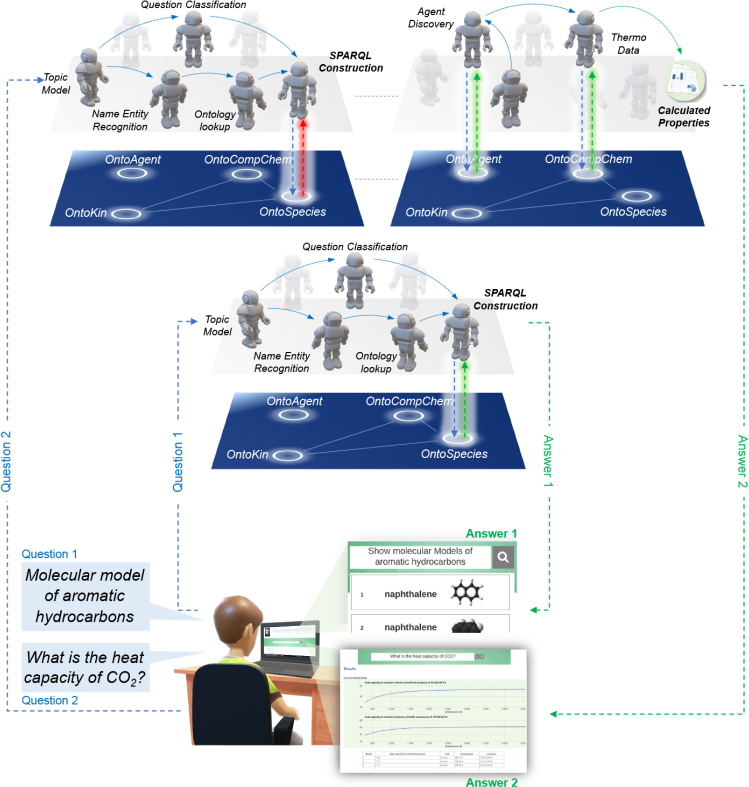
\includegraphics[height=1.50in,width=1.55in,viewport=0 0 750 790,clip]{Figures/TWA-KG-Marie.png}
%%\caption{\small\textrm{Mapping the relationship molecule (chemical) and synthon (abstract) concepts and illustrating them with instrances. cite from~\cite{ACR56-128_2023}}}%(与文献\cite{EPJB33-47_2003}图1对比)
%\label{Fig:Mapping-relationship-molecule-synthon}
%\end{figure}
%	\begin{itemize}
%{\fontsize{7.5pt}{5.5pt}\selectfont{
%		\item 以化合物为核心,借助语义网\textrm{(Semantic Web)},组织、表示和存储化学-化工和领域特定类型的知识
%		\item 构建拥有学习和推理能力,具备初级的创造知识的能力}}
%	\end{itemize}
%	\item 问-答式煤化工智能模型建设
%\begin{figure}[h!]
%\centering
%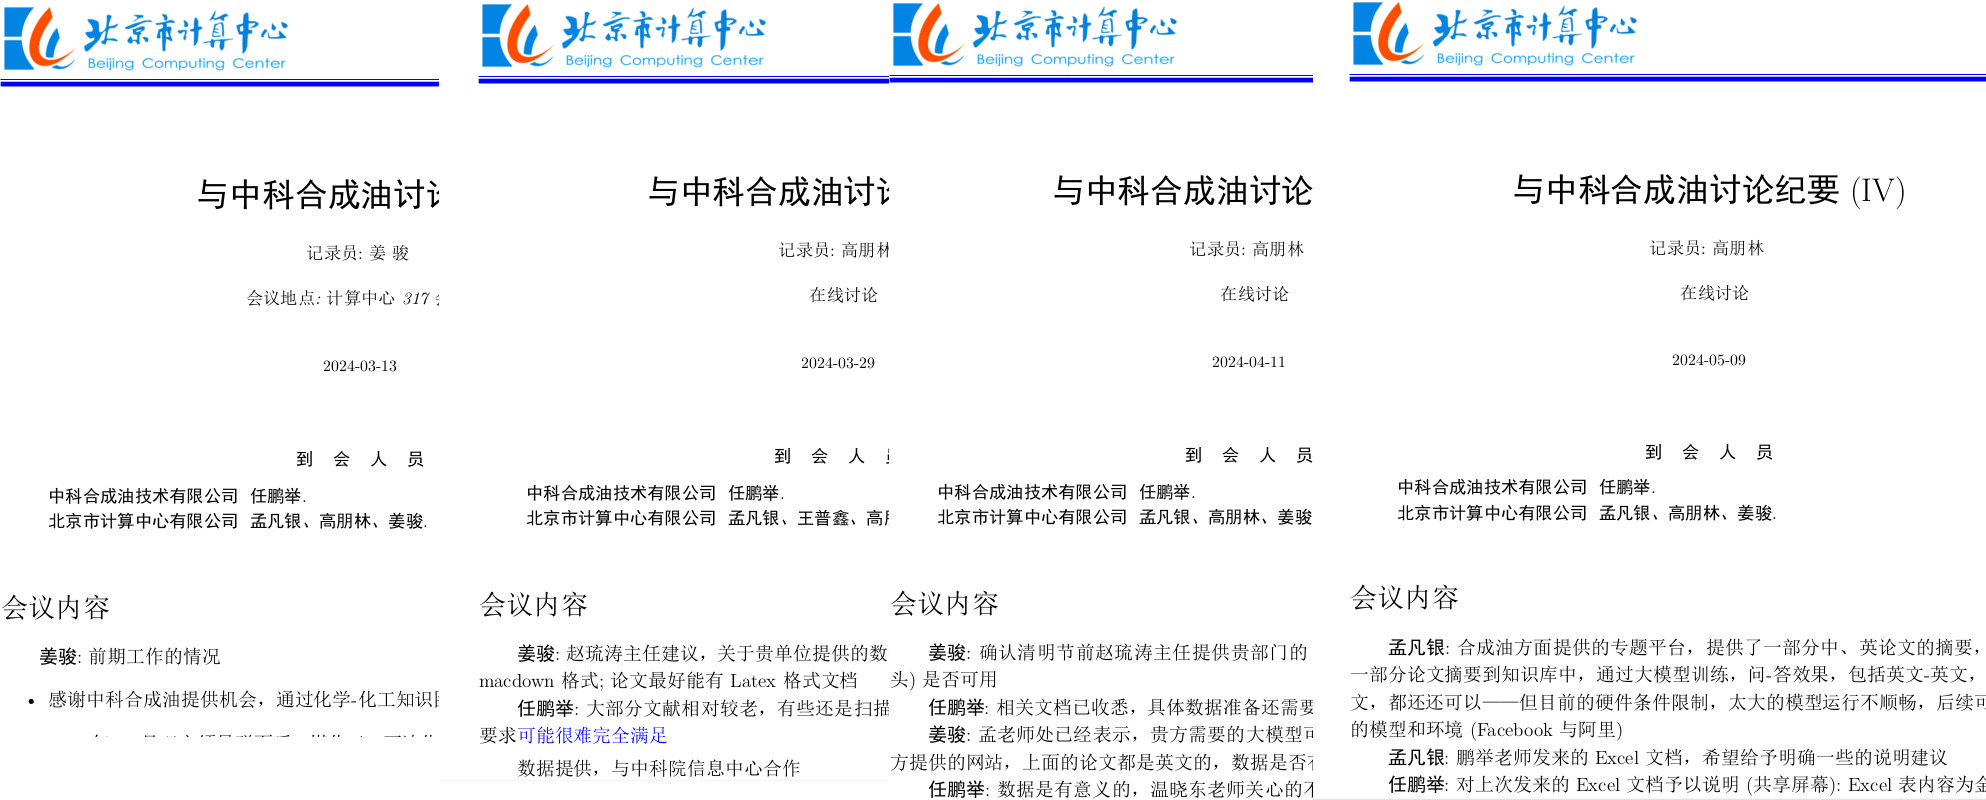
\includegraphics[height=1.40in,width=3.50in,viewport=0 0 1986 800,clip]{Figures/MeetingRecord_SCTC-BCC.png}
%\label{Fig:Meeting_Record}
%\end{figure}
%\begin{itemize}
%	\item 面向人工智能的全方位转型:\\
%		面向碳基础材料、发挥人工智能的作用
%	\item 大模型加持专业知识
%\end{itemize}
%	\end{itemize}
%\textcolor{purple}{目标:}~智能实验室-智能科学家
%\end{frame}
%
%\begin{frame}
%	\frametitle{数据驱动的材料研发:~应用前景}
%	\begin{enumerate}
%	 \setlength{\itemsep}{20pt}
%	 \item 航空发动机材料:~\textcolor{blue}{镍基单晶高温合金材料}\\
%	合金组分优化与强化功能提升
%
%\item 煤化工催化材料:~\textcolor{blue}{新型铁触媒材料}\\
%	反应活化性能提升与化学平衡的移动
%
%		\item 稀土功能材料:~\textcolor{blue}{钕铁硼永磁材料},\textcolor{blue}{稀土发光材料}\\
%	3\textit{d}-4\textit{f} 电子相互作用机制的认知
%
%	\end{enumerate}
%
%	\textcolor{magenta}{材料组分趋于复杂、材料机理认知趋于微观、材料与数据趋于膨胀}
%%\begin{figure}[h!]
%%\vspace*{-0.20in}
%%\centering
%%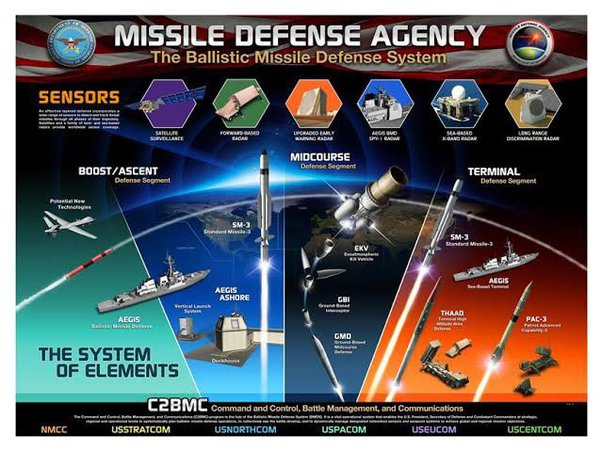
\includegraphics[height=2.90in,width=3.70in]{Figures/Main-qimg.jpeg}
%%\label{BMDS}
%%\end{figure}
%\end{frame}
%------------------------------------------------------------------------Reference----------------------------------------------------------------------------------------------
%		\frame[allowframebreaks]
%{
%\frametitle{主要参考文献}
%\begin{thebibliography}{99}
%{\tiny
%	\bibitem{PR136-B864_1964}\textrm{P. Hohenberg and W. Kohn, \textit{Phys. Rev.} \textbf{136} (1964), B864}
%	\bibitem{PR140-A1133_1965}\textrm{W. Kohn and L.J. Sham, \textit{Phys. Rev.} \textbf{140} (1965), A1133}
%	\bibitem{PRB50-17953_1994}\textrm{P. E. Bl\"ochl. \textit{Phys. Rev.} B, \textbf{50} (1994), 17953}
%	\bibitem{PRB59-1758_1999}\textrm{G. Kresse and D. Joubert \textit{Phys. Rev.} B, \textbf{59} (1999), 1758}
%	\bibitem{Elect_Stru}\textrm{Richard. M. Martin. \textit{Electronic Structure: Basic Theory and Practical Methods} (Cambridge University Press, Cambridge, England, 2004)}
%        \bibitem{Singh}\textrm{D. J. Singh. \textit{Plane Wave, PseudoPotential and the LAPW method} (Kluwer Academic, Boston,USA, 1994)}					%
%}
%\end{thebibliography}
%%\nocite*{}
%}

%\begin{figure}[h!]
%\vspace*{-0.20in}
%\centering
%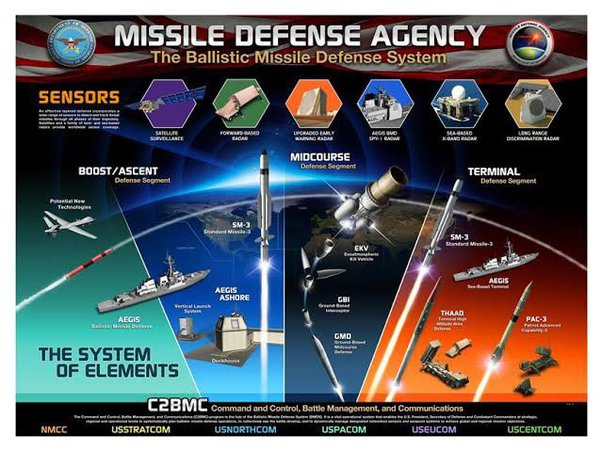
\includegraphics[height=2.90in,width=3.70in]{Figures/Main-qimg.jpeg}
%\label{BMDS}
%\end{figure}


\section{近期在研内容}
%\begin{frame}
%	\frametitle{近期研究任务}
%	自\textrm{2024}年起,团队与北京航空航天大学、北京科技大学、中科院宁波材料所等科研单位合作,联合承担的在研项目包括
%\begin{itemize}
%	\item \textcolor{blue}{国家自然基金面上项目}:\\
%	低维材料等离和激子极化激元的第一性原理研究%(项目编号: 12474217)}
%	\item \textcolor{blue}{科技部重大专项}:\\
%			基于人工智能技术的高性能多尺度分子动力学模拟平台%(项目编号: 2024ZD0606900)
%	\end{itemize}
%\end{frame}

\subsection{慢中子反应堆中氢化锆的原子扩散与辐照动力学}
\begin{frame}
	\frametitle{研究背景}
%锆合金
\begin{figure}[!ht]
\centering
\vspace*{-0.05in}
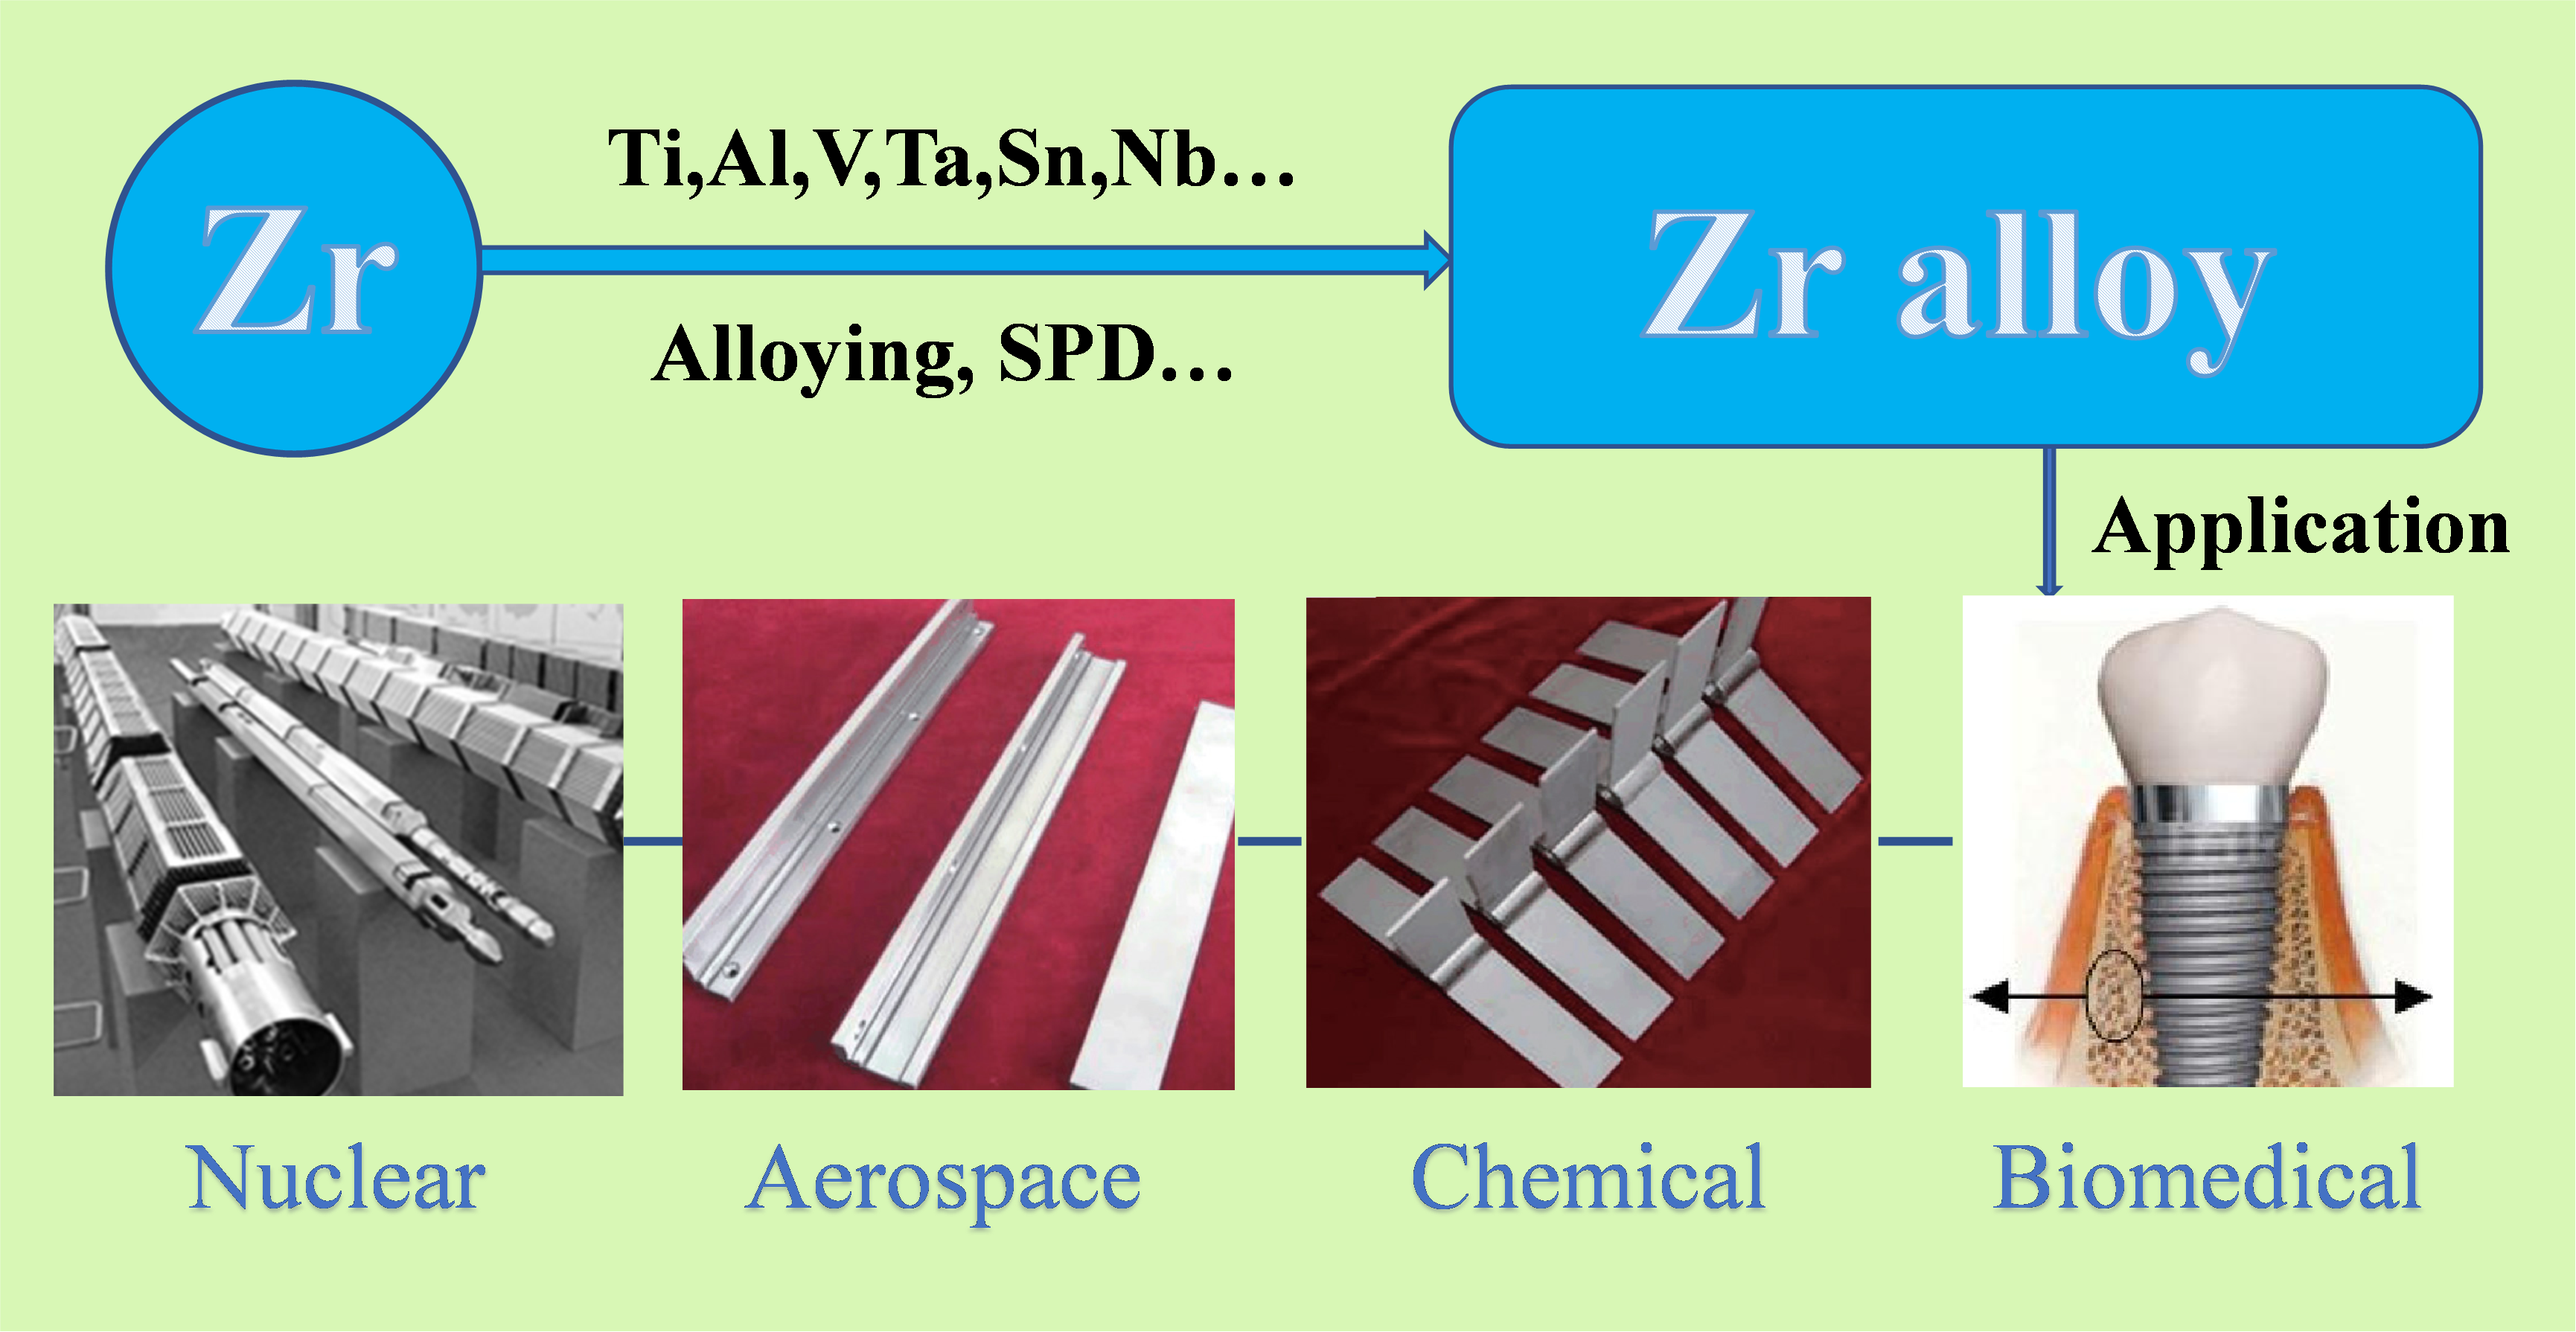
\includegraphics[height=1.45in,width=2.90in,viewport=0 0 430 230,clip]{Figures/Zr-Alloy_application.png}
%\vskip 0.10in
%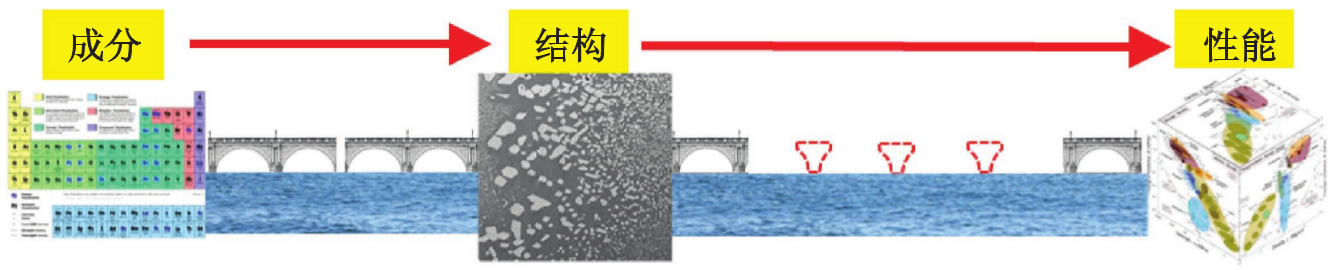
\includegraphics[height=0.85in]{Figures/Mat_Geno_Ene-3.png}
\caption{\tiny \textrm{Zr}-合金的主要应用.}
\label{Fig:Zr-Alloy_Application}
\end{figure}
\vskip -30pt
  \begin{columns}
	  \column{0.43\textwidth}
\begin{itemize}
	\item 热中子吸收截面:~\textcolor{blue}{低}
	\item 耐腐蚀性能:~\textcolor{blue}{优良}
	\item 结构与力学性能:~\textcolor{blue}{优异}
\end{itemize}
	  \column{0.58\textwidth}
\begin{itemize}
	\item 对\textrm{H}的亲和力极强%:~\textcolor{red}{极强}
	\item 氢化物易析出%:~\textcolor{\textrm{H}的溶解度极低}
	\item 包壳材料韧脆转变温度升高
\end{itemize}
  \end{columns}
\end{frame}

\begin{frame}
	\frametitle{慢中子堆中的氢化锆}
	氢化锆$(\mathrm{ZrH}_x)$在慢堆中的作用:~\textcolor{blue}{中子慢化剂}——提升反应堆的性能和安全性
	\begin{itemize}
		\item 氢化锆具有较高的慢化能力和较好的热稳定性,适用于小型反应堆和液态金属冷却的热中子反应堆
		\item 氢化锆具有较低的热中子吸收率,在熔盐堆中,可以显著提升反应堆的性能
		\item 氢化锆具有耐高温、抗辐照等特点,在高温环境下表现出色
	\end{itemize}
氢化锆中的氢易析出
\begin{itemize}
	\item 氢化锆作为中子慢化剂的工作温度在$650\sim750^{\circ}\mathrm{C}$
	%在该温度范围内,原子比大于$1.8$的氢化锆的氢分解压远远高于一个大气压
	\item 氢的析出将增大包壳中的气相压力
	\item 氢化锆中原子比减小(氢含量降低),会使其中子慢化能力减弱
	%,最终失去中子慢化的能力。
\end{itemize}
%与石墨相比,氢化锆在熔盐堆中具有较低的热中子吸收率,能够降低反应堆自持或增殖运行的难度
%氢化锆在慢堆中的具体应用场景包括:
%    小型反应堆:氢化锆适用于小型核反应堆,如空间堆,因为它能够在较高温度下工作而无需高压容器。
%    熔盐堆:在熔盐堆中,氢化锆作为慢化剂可以提升反应堆的安全性和经济性。通过优化氢锆原子比和熔盐体积比,可以改善熔盐堆的临界浓度和钍铀转换性能。
\end{frame}
%\section{研究目的和内容}
\begin{frame}
	\frametitle{研究目的}
%	\textcolor{red}{探索锆包壳材料接受辐照后损伤的微观动力学机理}:
%	\vskip 2pt
	通过理论计算研究氢化锆固体中\textcolor{blue}{氢原子}在高温、密闭真空环境的扩散行为,模拟实验结果
\begin{figure}[!ht]
\centering
\vspace*{-0.05in}
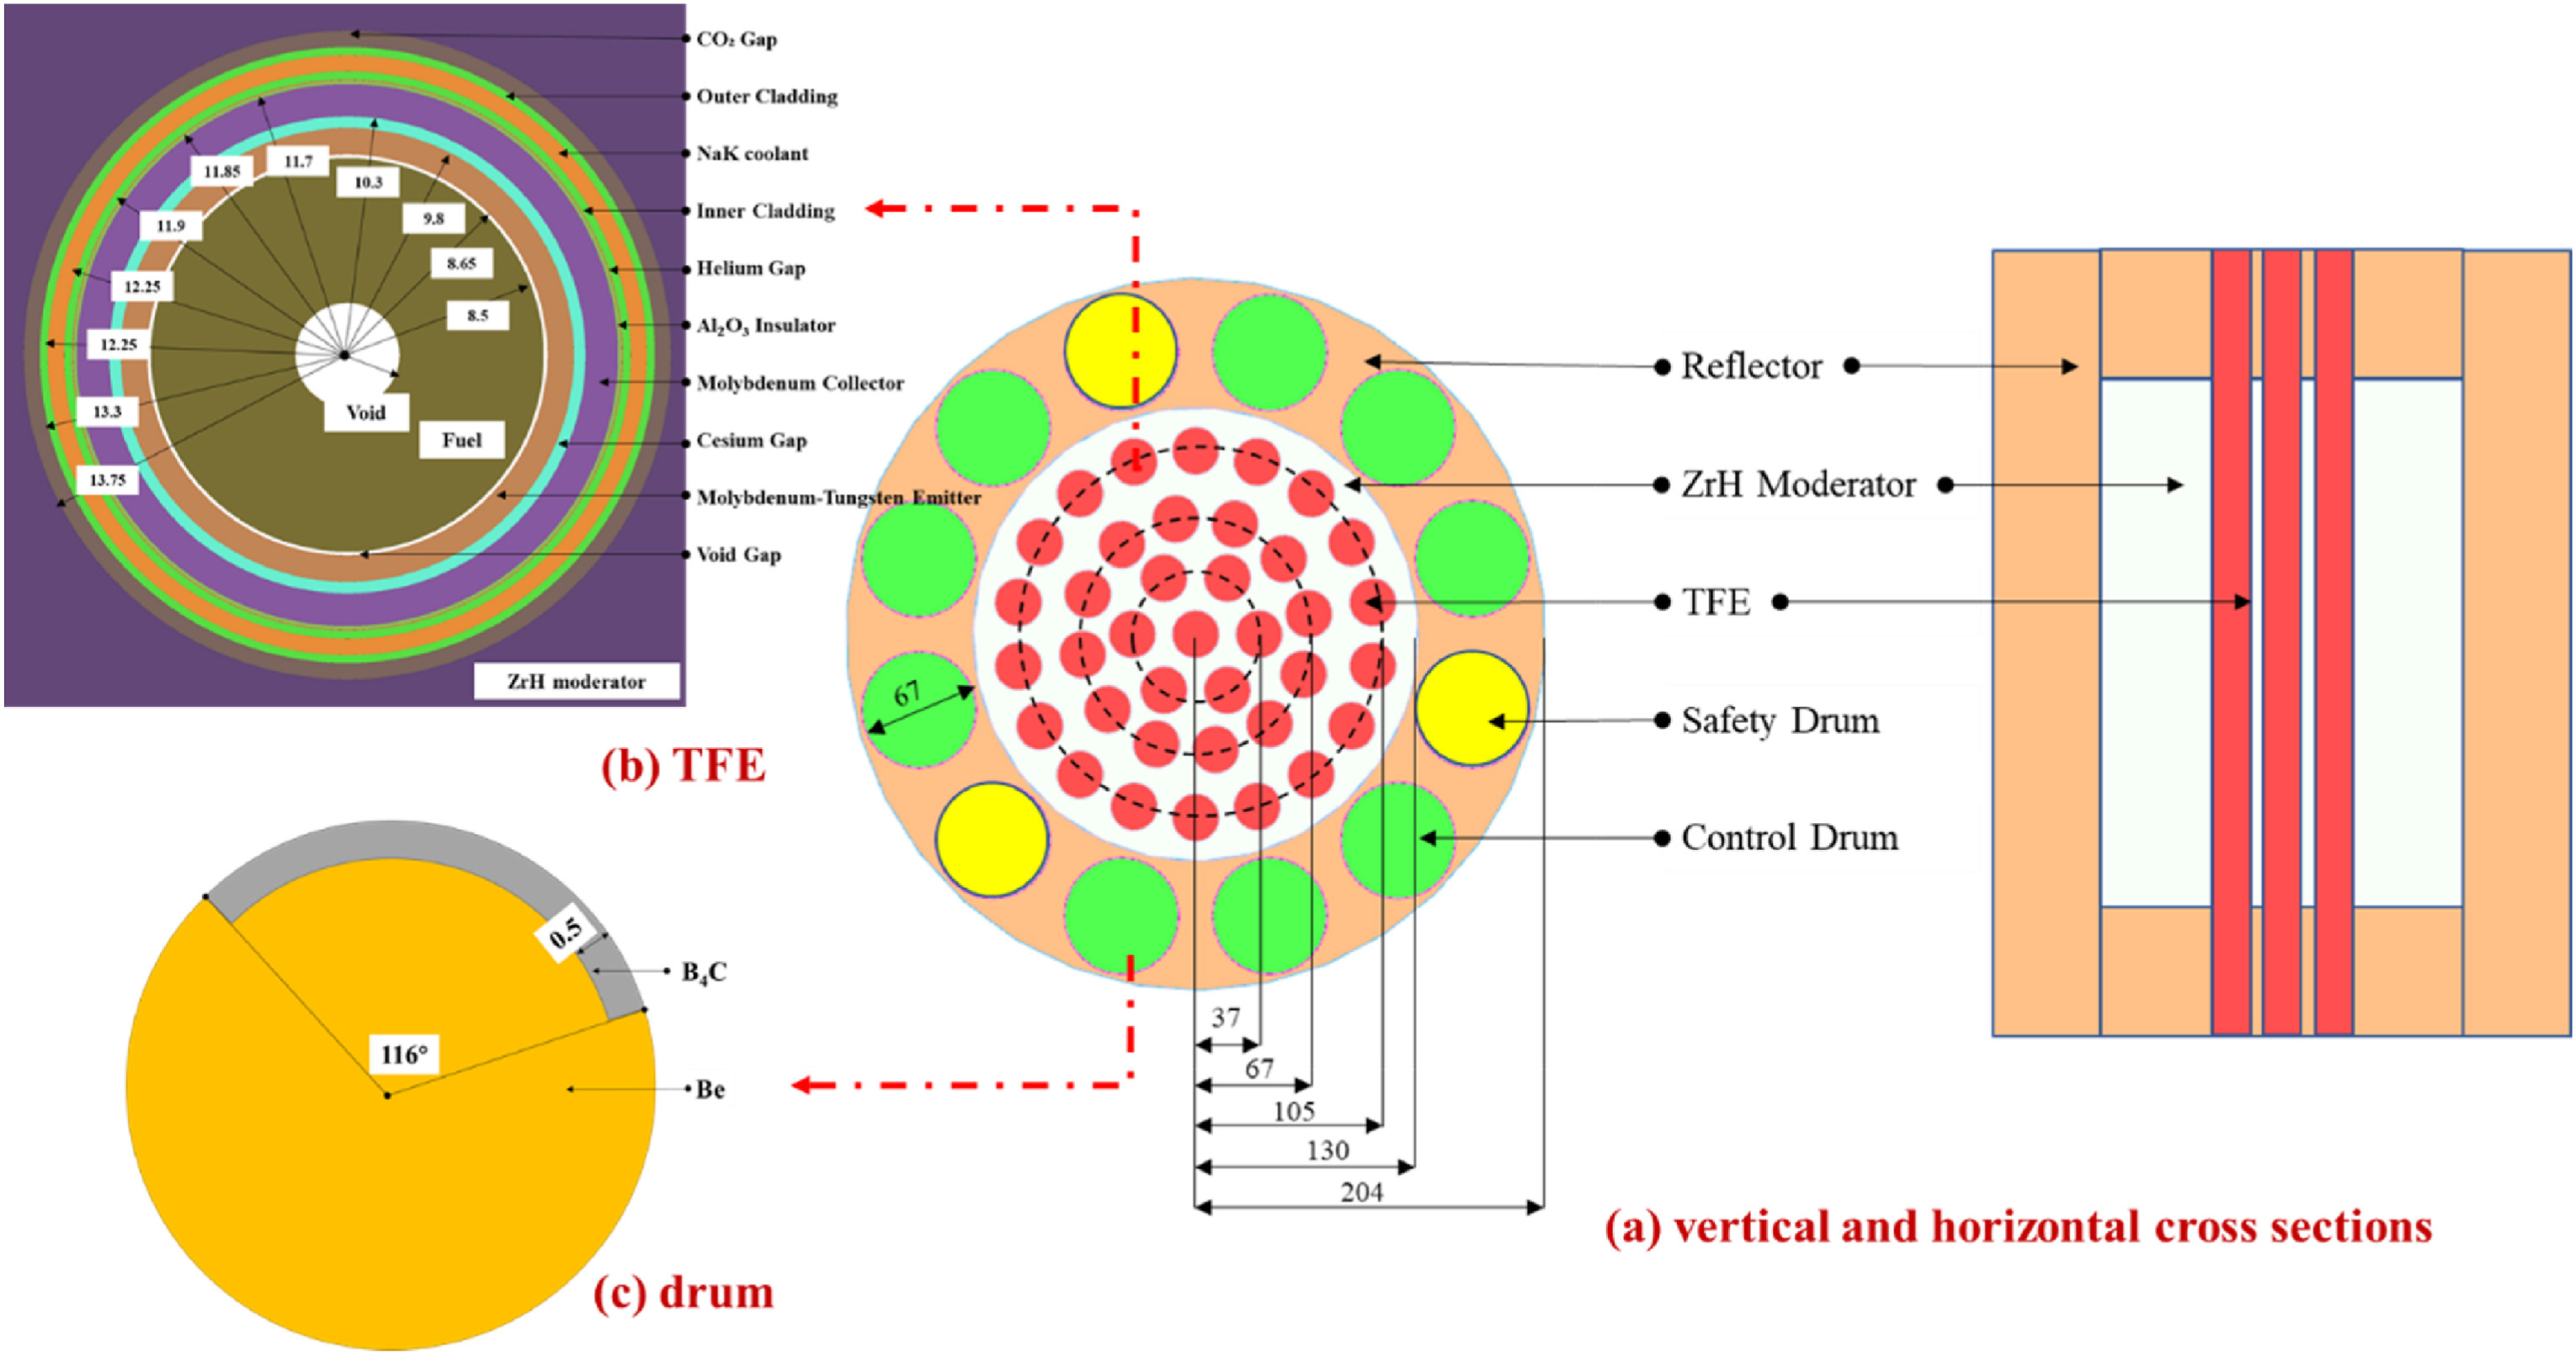
\includegraphics[height=1.40in,width=2.80in,viewport=0 0 450 240,clip]{Figures/Schematic_diagram_of_Topaz-II_reactor.jpeg}
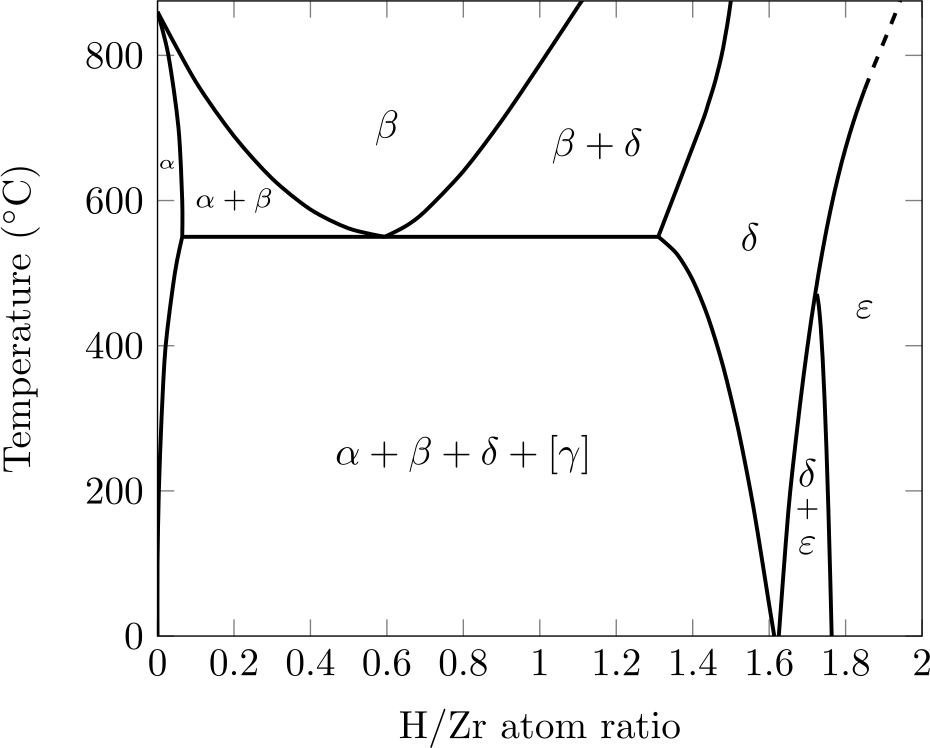
\includegraphics[height=1.20in,width=1.80in,viewport=0 0 930 748,clip]{Figures/Phase_diagram-Zr_H-systems.png}
\caption{\tiny \textrm{Phase diagram Zr-H systems.}}
\label{Fig:Phase_diagram-Zr_H-systems}
\end{figure}
\end{frame}

\begin{frame}
	\frametitle{氢化锆结构的多样性}
随着吸氢量的增加,锆合金中会先后形成
\begin{itemize}
	\item $\zeta$-氢化物\textrm{(\ch{Zr2H},HCP-密排六方结构)}
	\item \textcolor{blue}{$\gamma$-氢化物\textrm{(\ch{ZrH},FCT-面心四方结构)}}~\textcolor{red}{$\leftarrow$亚稳态}
	\item \textcolor{blue}{$\delta$-氢化物\textrm{(\ch{ZrH}$_{1.66}$,FCC-面心立方结构)}}~\textcolor{red}{$\leftarrow$稳态}
	\item $\varepsilon$-氢化物\textrm{(\ch{ZrH2},FCT-面心四方结构)}
\end{itemize}
\begin{figure}[!ht]
\centering
\vspace*{-0.05in}
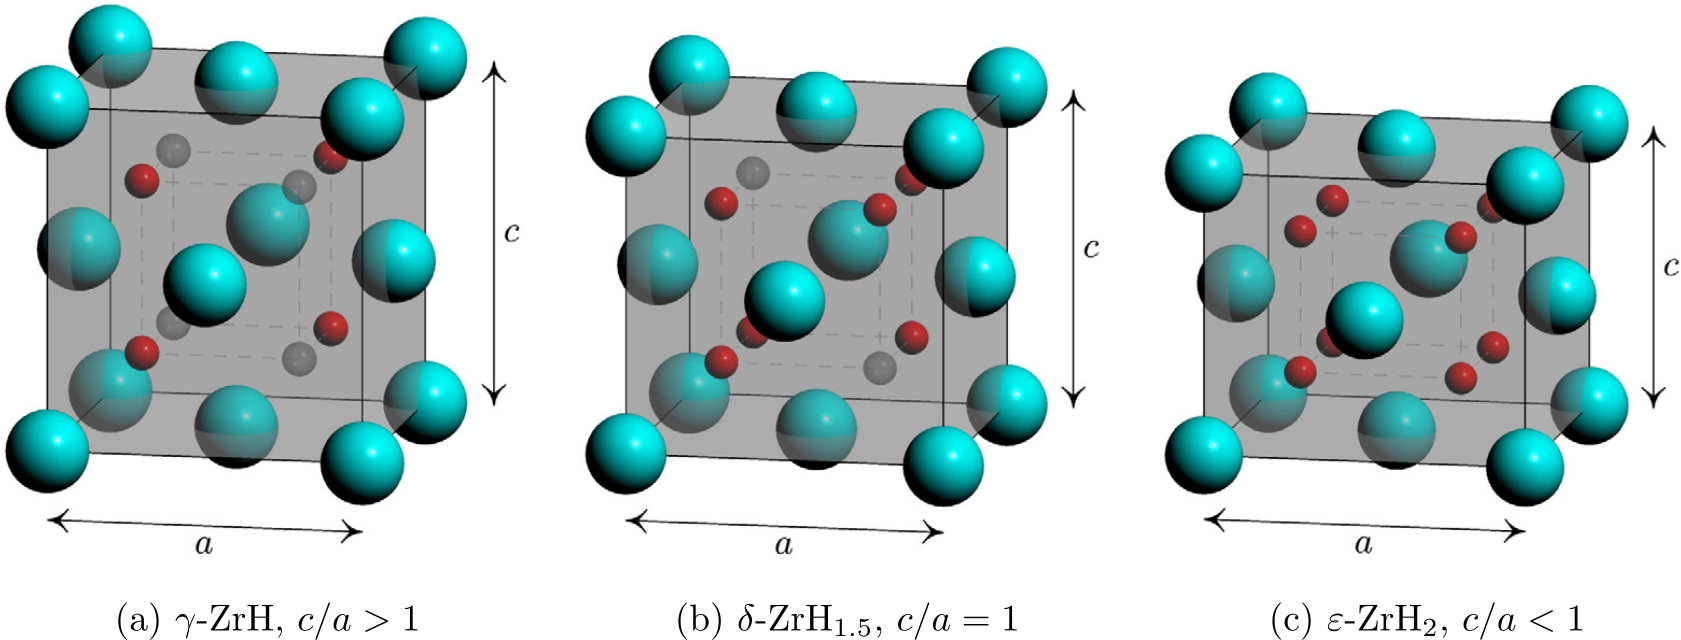
\includegraphics[height=1.50in,width=4.00in,viewport=0 0 1681 640,clip]{Figures/Characteristic_structures-for-the_ZrH_ZrH1.5_and_ZrH2-in-Zr_hydrides.png}
\caption{\tiny \textrm{Characteristic structures for the $\gamma$-ZrH, $\delta$-$\mathrm{ZrH}_{1.5}$, and $\varepsilon$-$\mathrm{ZrH}_2$ in Zr hydrides.}}
\label{Fig:Characteristic_structures-for-the_𝛾-ZrH_𝛿-ZrH1.5_and_𝜀-ZrH2-in-Zr_hydrides}
\end{figure}
%锆合金中常见的氢化物为$\gamma$氢化物和$\delta$氢化物,前者是亚稳态氢化物,后者为比较稳定的氢化物%。在没有外加应力的情况下,氢化物通常以锆基体的基面为惯习面,沿基面上的$<\mathrm{a}>$方向生长。在外加拉应力情况下,氢化锆会发生再取向,其惯习面会随着拉应力的增加逐步从基面转向\textrm{\{10-1$i$\} ($i$=1-7)}锥面,直至最后以柱面\{10-10\}为惯习面。再取向过程中,氢化物的生长方向始终沿着$<\mathrm{a}>$方向。在核燃料包壳管中,初始的氢化物都沿管子的周向分布,这与挤压管的初始织构密切相关,即锆包壳管具有基面沿管子周向分布的特征。在核反应堆服役过程中,核燃料在中子辐照下发生体积膨胀,使得包壳管被撑大,此时包壳管沿周向受到一定的拉应力,这种应力称之为环向应力\textrm{(hoop stress)}。在环向应力的作用下,当核反应堆冷却时,锆合金包壳管中的氢化物析出就会发生再取向,新的惯习面会沿着锥面或柱面。当环向拉应力超过\textrm{100~MPa}时,氢化物再取向主要会以柱面为惯习面。此时,若对比氢化物的初始分布和再取向分布,可以发现氢化物相当于转动了$90^{\circ}$,形成了大量的径向氢化物,沿锆合金包壳管厚度方向分布。这种再取向的氢化物会更容易造成锆合金包壳的失效。
\end{frame}

\begin{frame}
	\frametitle{研究内容}
	\begin{itemize}
	\item 氢化锆($\mathrm{ZrH}_{1.85-1.88}$)固体在高温(如$T=600^{\circ}\mathrm{C}$)密闭真空环境中,氢原子脱离氢化锆向外部空间中扩散的物理过程、扩散量及相应的扩散系数
	\item 氢化锆($\mathrm{ZrH}_{1.85-1.88}$)固体表面存在$\mathrm{ZrO}_2$涂层的条件下,氢原子脱离氢化锆向外部空间中扩散的物理过程、扩散量及相应的扩散系数
	\item 给定密闭空间体积,氢原子扩散后,整个扩散过程达到平衡时氢气的浓度
	\item 氢化锆($\mathrm{ZrH}_x$)固体中,不同浓度比例的氢(如$x=1.70$、$x=1.80$等)所对应的起始扩散温度
	\item 上述参数与表面$\mathrm{ZrO}_2$涂层的厚度的关系
	\end{itemize}
\end{frame}

%\section{研究方法}
\begin{frame}
	\frametitle{研究方法}
研究的主要难点是获得锆及原子的势函数,势函数是分子动力学模拟的基础,包括
  \begin{columns}
	  \column{0.35\textwidth}
\begin{itemize}
	\item $\mathrm{Zr}$-$\mathrm{Zr}$的势函数
	\item $\mathrm{Zr}$-$\mathrm{H}$的势函数
	\item $\mathrm{Zr}$-$\mathrm{O}$的势函数
	\item $\mathrm{H}$-$\mathrm{O}$势函数
\end{itemize}
	  \column{0.70\textwidth}
\begin{figure}[!ht]
\centering
\vspace*{-0.05in}
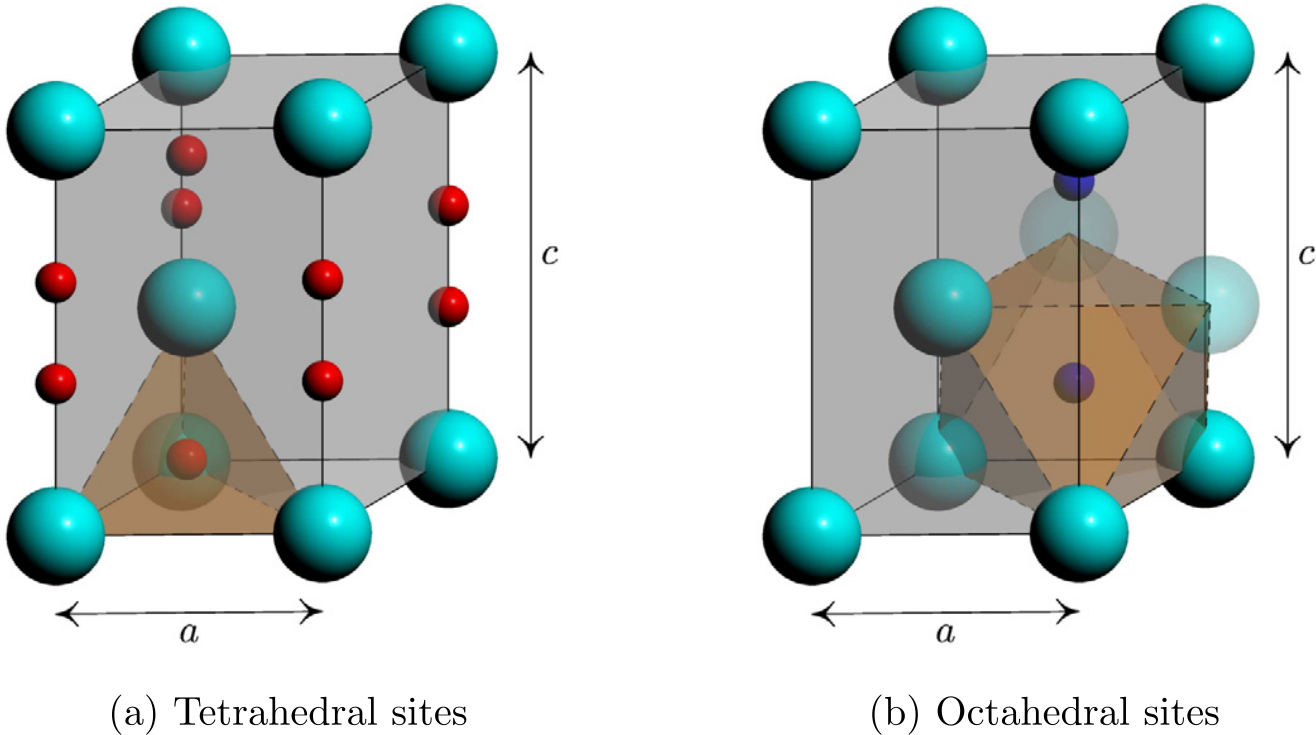
\includegraphics[height=1.20in,width=2.30in,viewport=0 0 1316 735,clip]{Figures/Interstitial_sites-used-by-H-for-occupancy-in-hcp_Zr.png}
\caption{\tiny \textrm{Interstitial sites used by H for occupancy in HCP Zr.}}
\label{Fig:Interstitial_sites-used-by-H-for-occupancy-in-hcp_Zr}
\end{figure}
  \end{columns}
每一类势函数构造需要至少\textrm{150}个百原子($10^2$量级)的模型,通过\textrm{DFT}计算获得基态能量和原子受力,总的原子模型约$10^3$量级,每次并发模型计算任务约为\textrm{5$\sim$20},平均每个模型计算时间为1天,以当前的计算资源估计,预计至少三-四个月完成相关模型的计算任务
\end{frame}

\begin{frame}
	\frametitle{机器学习势函数的构建}
%	构建\textrm{nep}势函数($\mathrm{Zr}$-$\mathrm{H}$势、$\mathrm{Zr}$-$\mathrm{O}$势)的主要步骤
	\begin{itemize}
		\item 准备各类所需的计算模型,完成模型的体系基态能量和原子受力的\textcolor{magenta}{\textrm{DFT}计算}
		\item 针对各模型,定义合适的\textcolor{blue}{描述符}:~与键长、键角和二面角相关
			{\fontsize{6.2pt}{4.2pt}\selectfont{\begin{displaymath}
				\begin{aligned}
					G_i^2=&\sum_{j\neq i}\mathrm{e}^{-\eta(r_{ij}-r_s)^2}f_c(r_{ij})\\
					G_i^3=&2^{1-\zeta}\sum_{j,k\neq i}(1+\lambda\cos\theta_{ijk})^{\zeta}\mathrm{e}^{-\eta(r_{ij}^2+r_{ik}^2+r_{jk}^2)}f_c(r_{ij})f_c(r_{ik})f_c(r_{jk})\\
					G_i^9=&2^{1-\zeta}\sum_{j,k\neq i}(1+\lambda\cos\theta_{ijk})^{\zeta}\mathrm{e}^{-\eta(r_{ij}^2+r_{ik}^2)}f_c(r_{ij})f_c(r_{ik})
				\end{aligned}
			\end{displaymath}}}
		\item 选定模型中的一部分结构及其能量和原子受力,应用机器学习方法(神经网络),用来\textcolor{magenta}{训练机器学习势}
		\item \textcolor{magenta}{优化}训练集的\textcolor{blue}{描述符},进一步改善机器学习势
		\item \textcolor{magenta}{评估并测试}产生的机器学习势
	\end{itemize}
\end{frame}
	
\begin{frame}
	\frametitle{神经网络势的训练}
	能量的表示
	\begin{displaymath}
		E_i=f_1^3\bigg\{b_1^3+\sum_{k=1}^{\mathrm{M}_{\mathrm{layer},2}}\omega_{n1}^{23}f_n^2\bigg[b_n^2+\sum_{m=1}^{\mathrm{M}_{\mathrm{layer},1}}\omega_{mn}^{12}f_m^1\bigg(b_m^1+\sum_{l=1}^{\mathrm{M}_{\mathrm{sym}}}\omega_{lm}^{01}G_{ij}\bigg)\bigg]\bigg\}
	\end{displaymath}
神经网络的优化函数
\begin{displaymath}
	\Gamma=\sum_{n=1}^{N_{\mathrm{struct}}}(E_{\mathrm{NN}}^n-E_{\mathrm{ref}}^n)^2+\beta^2\sum_{n=1}^{N_{\mathrm{struct}}}\sum_{m=1}^{3N_{\mathrm{atom}}^n}(F_{n,\mathrm{NN}}^m-F_{n,\mathrm{ref}}^m)^2
\end{displaymath}
\end{frame}

\begin{frame}
	\frametitle{计算任务进程:~\textrm{Zr-Zr}为例}
%	构造\textrm{Zr-Zr}相互作用势函数
	模型的来源与生产
	\begin{itemize}
		\item 由\textrm{Materials Project}选取一部分结构
		\item 通过\textrm{AIMD}模拟过程截取部分中间结构\textrm{(snapshots)}
	\end{itemize}
	计算模型的概况
	\begin{itemize}
		\item 模型类型:~\textrm{700$\sim$800}
		\item 每个模型:~约\textrm{120}原子
		\item 每个模型的\textrm{DFT}计算:~\textrm{64~cores}/\textrm{2.5~h}
	\end{itemize}
\end{frame}
%\appendix
%%------------------------------------------------------------------------Reference----------------------------------------------------------------------------------------------
%		\frame[allowframebreaks]
%		{
%\begin{thebibliography}{99}
%\frametitle{主要参考文献}
%{\tiny
%%	\bibitem{PhysCN40-477_2011}曹则贤, \textit{Secular,equation}, \textit{物理}, \textbf{40} \textrm{(2011), 477}
%	\bibitem{PR136-B864_1964}\textrm{P. Hohenberg and W. Kohn, \textit{Phys. Rev.} \textbf{136} (1964), B864}
%	\bibitem{PR140-A1133_1965}\textrm{W. Kohn and L.J. Sham, \textit{Phys. Rev.} \textbf{140} (1965), A1133}
%	\bibitem{JPC12-4409_1979}\textrm{J. Ihm, A. Zunger and L. Cohen, {\textit{J. Phys. C}} \textbf{12} (1979), 4409}
%	\bibitem{PRB41-7892_1990}\textrm{D. Vanderbilt. \textit{Phys. Rev.} B, \textbf{41} (1990), 7892} 
%	\bibitem{JPCM6-8245_1994}\textrm{G. Kresse and J. Hafner. J. Phys: \textit{Condens. Matter}, \textbf{6} (1994), 8245}
%	\bibitem{PRB50-17953_1994}\textrm{P. E. Bl\"ochl. \textit{Phys. Rev.} B, \textbf{50} (1994), 17953}
%	\bibitem{PRB59-1758_1999}\textrm{G. Kresse and D. Joubert \textit{Phys. Rev.} B, \textbf{59} (1999), 1758}
%	\bibitem{PRB12-3060_1975}\textrm{O. K. Andersen. \textit{Phys. Rev.} B, \textbf{12} (1975), 3060}
%	\bibitem{JMP22-2433_1981}\textrm{M. Weiner. \textit{J. Math. Phys.}, \textbf{22} (1981), 2433}
%	\bibitem{PRB26-4571_1982}\textrm{M. Weinert, E. Wimmer and A. J. Freeman. \textit{Phys. Rev.} B, \textbf{26} (1982), 4571}
%	\bibitem{Andersen_Book}\textrm{O. K. Andersen. \textit{Computational Methods in Band Theory} (Plenum, New York, USA, 1971)}
%        \bibitem{Singh}\textrm{D. J. Singh. \textit{Plane Wave, PseudoPotential and the LAPW method} (Kluwer Academic, Boston,USA, 1994)}					%
%	\bibitem{Singh}\textrm{D. J. Singh. \textit{Plane Wave, PseudoPotential and the LAPW method} (Kluwer Academic, Boston,USA, 1994)}
%	\bibitem{Xie-Lu}谢希德、陆栋\:主编, {\textit{固体能带理论}}\:复旦大学出版社, 上海, 1998
%	\bibitem{Nemoshkalenko-Antonov}\textrm{V. V. Nemoshkalenko and V. N. Antonov. \textit{Computational Methods in Solid State Physics} (Gordon and Breach Science Publisher, Amsterdam, The Netherlands, 1998)}
%	\bibitem{Elect_Stru}\textrm{Richard. M. Martin. \textit{Electronic Structure: Basic Theory and Practical Methods} (Cambridge University Press, Cambridge, England, 2004)}
%	\bibitem{Xu_Li_Wang}徐光宪、黎乐民、王德民, {\textit{量子化学——基本原理和从头计算法}}\;\textrm{({\textit{上、中}})}\:科学出版社, 北京, 1980
%%	\bibitem{SSC114-15_2000}\textrm{E. Sj\"ostedt, L. Nordstr\"om and D. J. Singh. \textit{Solid State Commun.}, \textbf{114} (2000), 15}
%}
%\end{thebibliography}
%\nocite*{}
%}
	\subsection{$\mathrm{CO}_2$还原的催化机理}
\begin{frame}[allowframebreaks]
	\frametitle{$\mathrm{CO}_2$还原为$\mathrm{CO}$后继续加\textrm{H}的反应机理}
%	{\huge
%		\setchemfig{atom sep=2em, bond style={line width=1pt, red, dash pattern=on 2pt off 2pt}}
%		\chemname{\chemfig{H-C(-[2]H)(-[6]H)-C(=[1]O)-[7]H}}{Acetaldehyde}}
	为了检验\textrm{\ch{CO}}与\textrm{H}的反应历程,设计方案
\begin{itemize}
	\item \textrm{\ch{CO}}加\textrm{\ch{H}}的能力:\\加在\textrm{\ch{C}}端(生成\textrm{\chemfig{H-[,0.3]C(=[1,0.7]O)-[6,0.3]}})%\chemfig{R-[:30]*-[:180]H}\\
		~\textrm{\textcolor{blue}{vs}}~加在\textrm{\ch{O}}端(生成\textrm{\chemfig{C(=[1,0.7]O-[,0.3]H)(-[5,0.3])-[7,0.3]}})
	\item 类比\textrm{\ch{CN}}和\textrm{\ch{NO}}的两端加\textrm{\ch{H}}能力
	\item 系统类比加\textrm{\ch{H}}引起体系能量和电荷密度的变化
\end{itemize}
\begin{figure}[h!]
\centering
\begin{tikzpicture}[
%    box/.style={rectangle,draw,node distance=1cm,text width=15em,text centered,rounded corners,minimum height=2em,thick},  %文字居中
    box/.style={rectangle,draw,node distance=1cm,text width=18em,anchor=west,rounded corners,minimum height=5em,thick},   %文字左对齐
    arrow/.style={draw,-latex', red, line width=2pt},
]
\node [box](box){};
\node [anchor=west, text width=1em] (H1) {\textrm{\ch{H}}};  %% anchor=west 文字左对齐
\node [right=2 of H1] (CO) {\textrm{\chemfig{C~O}}};
\path [arrow, draw=red, line width =0.5pt] (10.5em,0.2em) -- (8.5em, 0.2em);
\node [right=5.5 of H1] (H2) {\textrm{\ch{H}}};
\node [above=0.05 of CO] (CN) {\textrm{\chemfig{C(~N)}}};
\draw [draw=red] (7.6em,1.6em) circle [radius=0.1em];
\node [below=0.05 of CO] (NO) {\textrm{\chemfig{N(=O)}}};
\filldraw [fill=red, draw=red] (9.6em,-1.2em) circle [radius=0.1em];
\filldraw [fill=red, draw=red] (11.7em,-1.4em) circle [radius=0.1em];
\filldraw [fill=red, draw=red] (11.7em,-1.8em) circle [radius=0.1em];
% \path [arrow] (Method) -- (Softwares);
  \path [arrow, dotted] (CO) -- (H1);
  \path [arrow, draw=blue, dotted] (CO) -- (H2);
\end{tikzpicture}
\caption{\tiny{\textrm{\ch{CO}、\ch{CN}、\ch{NO}}分子两端加\textrm{\ch{H}}的示意,不同距离的\textrm{X-H~(X=C、N、O)},示意加\textrm{H}的动力学过程}}
\label{Molecules}
\end{figure}
反应模型:~活化的\textrm{\ch{CO}}与\textrm{\ch{H}}
\begin{figure}[h!]
\centering
%\vspace*{-0.10in}
\includegraphics[height=2.00in,width=1.9in, viewport=1870 350 2950 1500, clip]{/home/jun-jiang/BCC/2023-NICE/Ni-CO2/图片/能量测试结构/活化C-O---H.png}
\includegraphics[height=2.00in,width=1.9in, viewport=1870 350 2950 1500, clip]{/home/jun-jiang/BCC/2023-NICE/Ni-CO2/图片/能量测试结构/活化H---C-O.png}
\caption{\tiny \textrm{The front view of model for \ch{CO}-activated compounded with \ch{H} by \ch{O}-end (left) and \ch{C}-end (right).}}%(与文献\cite{EPJB33-47_2003}图1对比)
\label{Model:CO-H}
\end{figure}
反应模型:~活化的\textrm{\ch{CN}}与\textrm{\ch{H}}
\begin{figure}[h!]
\centering
%\vspace*{-0.10in}
\includegraphics[height=2.00in,width=1.9in, viewport=1870 350 2950 1500, clip]{/home/jun-jiang/BCC/2023-NICE/Ni-CO2/图片/能量测试结构/活化C-N---H.png}
%\includegraphics[height=2.00in,width=1.9in, viewport=1870 350 2950 1500, clip]{/home/jun-jiang/BCC/2023-NICE/Ni-CO2/图片/能量测试结构/活化H---C-O.png}
\caption{\tiny \textrm{The front view of model for \ch{CN}-activated compounded with \ch{H} by \ch{N}-end.}}%(与文献\cite{EPJB33-47_2003}图1对比)
\label{Model:CN-H}
\end{figure}
反应模型:~活化的\textrm{\ch{NO}}与\textrm{\ch{H}}
\begin{figure}[h!]
\centering
%\vspace*{-0.10in}
\includegraphics[height=2.00in,width=1.9in, viewport=1870 350 2950 1500, clip]{/home/jun-jiang/BCC/2023-NICE/Ni-CO2/图片/能量测试结构/活化N-O---H.png}
\includegraphics[height=2.00in,width=1.9in, viewport=1870 350 2950 1500, clip]{/home/jun-jiang/BCC/2023-NICE/Ni-CO2/图片/能量测试结构/活化H---N-O.png}
\caption{\tiny \textrm{The front view of model for \ch{NO}-activated compounded with \ch{H} by \ch{O}-end (left) and \ch{N}-end (right).}}%(与文献\cite{EPJB33-47_2003}图1对比)
\label{Model:NO-H}
\end{figure}

差分电荷表示:~活化的\textrm{\ch{CO}}与\textrm{\ch{H}}反应
\begin{figure}[h!]
\centering
%\vspace*{-0.10in}
\includegraphics[height=2.00in,width=1.9in, viewport=1870 850 2950 1880, clip]{/home/jun-jiang/BCC/2023-NICE/Ni-CO2/图片/差分电荷/俯视活化C-O---H.png}
\includegraphics[height=2.00in,width=1.9in, viewport=1870 480 2950 1780, clip]{/home/jun-jiang/BCC/2023-NICE/Ni-CO2/图片/差分电荷/正视活化C-O---H.png}
\caption{\tiny \textrm{The top-view (left) and front-view (right) of charge-density difference for \ch{CO}-activated compounded with \ch{H}.}}%(与文献\cite{EPJB33-47_2003}图1对比)
\label{Charge-density_difference:CO}
\end{figure}
差分电荷表示:~活化的\textrm{\ch{NO}}与\textrm{\ch{H}}反应
\begin{figure}[h!]
\centering
%\vspace*{-0.10in}
\includegraphics[height=2.00in,width=1.9in, viewport=1870 850 2950 1880, clip]{/home/jun-jiang/BCC/2023-NICE/Ni-CO2/图片/差分电荷/俯视活化N-O---H.png}
\includegraphics[height=2.00in,width=1.9in, viewport=1870 480 2950 1780, clip]{/home/jun-jiang/BCC/2023-NICE/Ni-CO2/图片/差分电荷/正视活化N-O---H.png}
\caption{\tiny \textrm{The top-view (left) and front-view (right) of charge-density difference for \ch{NO}-activated compounded with \ch{H}.}}%(与文献\cite{EPJB33-47_2003}图1对比)
\label{Charge-density_difference:NO}
\end{figure}
能量-键长呈现的反应动力学可能性
\begin{figure}[h!]
\centering
%\vspace*{-0.10in}
\includegraphics[height=2.10in,width=4.0in, viewport=0 0 360 200, clip]{/home/jun-jiang/BCC/2023-NICE/Ni-CO2/X-H_E.eps}
\caption{\tiny 金属表面吸附的\textrm{\ch{CO}、\ch{CN}、\ch{NO}}分子与\textrm{\ch{H}}相互作用的能量随\textrm{X-H~(X=C、N、O)}间距的变化}%\textrm{The energy of  of \ch{CO2} activation over \ch{Ni}.}}%(与文献\cite{EPJB33-47_2003}图1对比)
\label{X-H_E}
\end{figure}
\newpage
对比金属表面吸附的\textrm{\ch{CN}}、\textrm{\ch{CO}}、\textrm{\ch{NO}}
\begin{itemize}
	\item \textrm{\ch{CO}}更明显地倾向\textrm{\ch{C}}端与\textrm{\ch{H}}优先反应
%	\item \textrm{\ce{CO2->[+H2]COOH}\ce{->[-H2O]CO}\ce{->[+H2]COH}}
	\item \textrm{\ce{CO2 ->[\ce{+H2}] COOH ->[\ce{-H2O}] CO ->[\ce{+H2}] \chemfig{H-[,0.3]C(=[1,0.7]O)-[6,0.3]} ->[\ce{+H2}] $\cdots$ -> CH4}}
\end{itemize}

\end{frame}

\frame
{
	\frametitle{其他成果与论著}
\begin{itemize}
	\item {\fontsize{8.2pt}{6.2pt}\selectfont{\textcolor{red}{国家自然科学基金}~\textcolor{blue}{``低维材料等离和激子极化激元的第一性原理研究''}}}
%		{\fontsize{8.2pt}{4.2pt}\selectfont{(项目批准号:~\textrm{12474217})}}
%		\vskip 1pt
%		{\fontsize{8.2pt}{6.2pt}\selectfont{(项目持续年度:~ \textrm{2025.01-2028.12})}}
	\item {\fontsize{8.2pt}{6.2pt}\selectfont{\textcolor{red}{新材料研发及应用国家重大专项}~\textcolor{blue}{``基于人工智能技术的高性能多尺度分子动力学模拟平台''项目}}}
\end{itemize}
\begin{itemize}
%	\setlength{\itemsep}{1pt}
	\item {\fontsize{8.0pt}{4.2pt}\selectfont{\underline{赵琉涛}, \underline{姜骏}, \underline{王彩群}, 潘勇, 潘震西, \textcolor{blue}{计算材料科学理论与实践}, 人民邮电出版社, (北京), 2021}}
\end{itemize}
\begin{figure}[h!]
\centering
\vskip -5pt
\includegraphics[height=1.7in,width=1.3in]{Figures/Cover-Computing_Materials.jpg}
\label{Fig:Cover}
%\caption{\fontsize{5.2pt}{6.2pt}\selectfont{$\vec k\cdot\vec p$方法保证计算精度,并计算效率提升}}%
\end{figure}
}

\begin{frame}
	\frametitle{其他成果与论著}
	\begin{itemize}
		\item {\fontsize{5.2pt}{1.2pt}\selectfont{\textrm{Zhenxi Pan, Yong Pan, \underline{Jun Jiang} and \underline{Liutao Zhao}$^{\dagger}$, \textcolor{blue}{High-Throughput Electronic Band Structure Calculations for Hexaborides}, \textit{CompCom~2019 AIOSC}, \textbf{998}, (2019), 386-395}}}
		\item {\fontsize{5.2pt}{1.2pt}\selectfont{\textrm{Yurui Wang, Zhihui Du$^{\dagger}$, \underline{Jun Jiang}, Baokun Lu and Chongyu Wang, \textcolor{blue}{Modeling the Parallel Efficiency of Density Functional Theory based Jobs on Sunway TaihuLight}, \textit{2019 IEEE-CSE and IEEE-EUC}, (2019), 199-204}}}
		\item {\fontsize{5.2pt}{1.2pt}\selectfont{\textrm{Zhihui Du$^{\dagger}$, Xinning Hui, Yurui Wang, \underline{Jun Jiang}, Jason Liu, Baokun Lu and Chongyu Wang, \textcolor{blue}{Inter-Job Scheduling of High-Througput Material Screening Applications}, \textit{2020 IPDPS}, (2020), 841-852}}}
		\item {\fontsize{5.2pt}{1.2pt}\selectfont{\textrm{Jianxin Huang, Jinkai Wang, Hao Wang$^{\dagger}$, Jiajun Lu, Xiao-Gang Lu, \underline{Jun Jiang} and Ying Chen, \textcolor{blue}{Influences of multicenter bonding and interstitial elements on psudo-twinned $\gamma$-\ch{TiAl} crystal}, \textit{Phys. Scr.}, \textbf{97}, (2022), 085403}}}
		\item {\fontsize{5.2pt}{1.2pt}\selectfont{\textrm{\underline{Caiqun Wang}, \underline{Penglin Gao}, \underline{Hongfei Li}, Mei Yang, \underline{Jun Jiang}, \underline{Liutao Zhao} and Ping Qian$^{\dagger}$, \textcolor{blue}{Single-atom catalysts:~Effects of end-group regulation on catalytic activity}, \textit{Mater. Tod. Comm..}, \textbf{40}, (2024), 109482}}}
	\end{itemize}
\end{frame}
%\section{第一原理材料计算核心软件研究}
\begin{frame}
	\frametitle{小结}
	\begin{itemize}
	\setlength{\itemsep}{5pt}
		\item 团队基于材料计算结合人工智能和数据驱动的尝试是有效的
		\item 团队的研究工作依然处于起步阶段,各方面工作都有待深入和完善
		\item 团队成员与高校、科研院所的交流有待加强
		\item 团队的组织和研发模式需要探索\\
			{\fontsize{8.2pt}{6.2pt}\selectfont{研发重点面向基础科研的应用领域,一方面相关研究工作对计算资源的需求较大、产品和成果的市场化程度低,但同时相关领域研究的自主可控需求程度高,需要探索研究应用-市场需求的平衡}}
	\end{itemize}
	\huge\textcolor{red}{衷心感谢中心领导对团队的支持}
\end{frame}
%\frame
%{
%	\frametitle{专利}
%	\begin{itemize}
%		\item {\fontsize{7.5pt}{6.2pt}\selectfont{\underline{姜骏}, 王崇愚, 晶体对称性及能带路径确定方法及装置}}
%	\end{itemize}
%\begin{figure}[h!]
%\centering
%\vskip -5pt
%\includegraphics[height=2.3in,width=1.6in]{Figures/Certificate-of-Patent.png}
%\label{Fig:Patent}
%%\caption{\fontsize{5.2pt}{6.2pt}\selectfont{$\vec k\cdot\vec p$方法保证计算精度,并计算效率提升}}%
%\end{figure}
%}
%
%------------------------------------------------------------------------Reference----------------------------------------------------------------------------------------------
%		\frame[allowframebreaks]
%{
%\frametitle{主要参考文献}
%\begin{thebibliography}{99}
%{\tiny
%	\bibitem{PR136-B864_1964}\textrm{P. Hohenberg and W. Kohn, \textit{Phys. Rev.} \textbf{136} (1964), B864}
%	\bibitem{PR140-A1133_1965}\textrm{W. Kohn and L.J. Sham, \textit{Phys. Rev.} \textbf{140} (1965), A1133}
%	\bibitem{PRB50-17953_1994}\textrm{P. E. Bl\"ochl. \textit{Phys. Rev.} B, \textbf{50} (1994), 17953}
%	\bibitem{PRB59-1758_1999}\textrm{G. Kresse and D. Joubert \textit{Phys. Rev.} B, \textbf{59} (1999), 1758}
%	\bibitem{Elect_Stru}\textrm{Richard. M. Martin. \textit{Electronic Structure: Basic Theory and Practical Methods} (Cambridge University Press, Cambridge, England, 2004)}
%        \bibitem{Singh}\textrm{D. J. Singh. \textit{Plane Wave, PseudoPotential and the LAPW method} (Kluwer Academic, Boston,USA, 1994)}					%
%}
%\end{thebibliography}
%%\nocite*{}
%}
%-----------------------------------------------------------------------------------------------------------------------------------------------------------------------%

